\documentclass[14pt,letterpaper]{article}

% ============ Page Layout ============
\usepackage[margin=1in]{geometry}
\usepackage{fancyhdr}
\pagestyle{fancy}
\fancyhf{}
\rhead{Midterm Review}
\lhead{Onur Calisir}
\rfoot{Page \thepage}

% ============ Math Packages ============
\usepackage{amsmath, amssymb, amsthm}
\usepackage{mathtools}  % Enhanced math (e.g., dcases)
\usepackage{bm}         % Bold math symbols (\bm{x})
\usepackage{bbm}        % Blackboard bold for indicators
% \usepackage{algorithm2e}  % for algorithms

% ============ Graphics & Figures ============
\usepackage{graphicx}
\usepackage{tikz}
\usetikzlibrary{bayesnet, arrows.meta, positioning}
\usepackage{float}
\usepackage{tcolorbox}    % for colored boxes
\usepackage{xcolor}      % For colors
\usepackage{colortbl}    % For \rowcolor
% ============ Algorithms ============
\usepackage[ruled,vlined,linesnumbered]{algorithm2e}
\SetKwInput{KwInput}{Input}
\SetKwInput{KwOutput}{Output}

% ============ Code Blocks ============
\usepackage{listings}
\usepackage{xcolor}

\definecolor{codegreen}{rgb}{0,0.6,0}
\definecolor{codegray}{rgb}{0.5,0.5,0.5}
\definecolor{codepurple}{rgb}{0.58,0,0.82}
\definecolor{backcolour}{rgb}{0.95,0.95,0.92}

\lstdefinestyle{mystyle}{
    backgroundcolor=\color{backcolour},
    commentstyle=\color{codegreen},
    keywordstyle=\color{magenta},
    numberstyle=\tiny\color{codegray},
    stringstyle=\color{codepurple},
    basicstyle=\ttfamily\footnotesize,
    breakatwhitespace=false,
    breaklines=true,
    captionpos=b,
    keepspaces=true,
    numbers=left,
    numbersep=5pt,
    showspaces=false,
    showstringspaces=false,
    showtabs=false,
    tabsize=2
}
\lstset{style=mystyle}

% ============ Theorem Environments ============
\theoremstyle{definition}
\newtheorem{definition}{Definition}[section]
\newtheorem{theorem}{Theorem}[section]
\newtheorem{lemma}{Lemma}[section]
\newtheorem{corollary}{Corollary}[section]
\newtheorem{example}{Example}[section]

% ============ Custom Commands ============
% Probability & Statistics
\newcommand{\expect}[1]{\mathbb{E}\left[#1\right]}
\newcommand{\var}[1]{\text{Var}\left(#1\right)}
\newcommand{\cov}[2]{\text{Cov}\left(#1, #2\right)}

% Distributions
\newcommand{\normal}[2]{\mathcal{N}\left(#1; #2\right)}
\newcommand{\uniform}[2]{\mathcal{U}\left(#1; #2\right)}

% Shortcuts
\newcommand{\pcond}[2]{p(#1 \mid #2)}

% State space notation
\newcommand{\state}{\bm{x}}
\newcommand{\obs}{\bm{z}}
\newcommand{\control}{\bm{u}}
\newcommand{\noise}{\bm{w}}
\newcommand{\dt}{\Delta t}
\DeclareMathOperator*{\argmax}{arg\,max}
\DeclareMathOperator*{\argmin}{arg\,min}

\DeclareMathOperator{\atantwo}{atan2}
% ============ Hyperlinks ============
\usepackage[colorlinks=true, linkcolor=blue, citecolor=blue, urlcolor=blue]{hyperref}

% ============ Title Info ============
\title{Probabilistic Robotics - Midterm Study Notes}
\author{Onur Calisir}
\date{\today}

\begin{document}
\maketitle
% \tableofcontents
\newpage
% ============================================================================
% BAYES FILTER - EXAM NOTES
% Optimized for open-book exam: Quick reference + complete derivations
% ============================================================================

\section{Quick Reference: Bayes Filter}

\begin{tcolorbox}[colback=yellow!10!white,colframe=orange!75!black,title=\textbf{Bayes Filter - Fast Reference}]
\textbf{Purpose:} Recursive state estimation from noisy sensors and imperfect control

\vspace{2mm}
\textbf{Required Models:}
\begin{itemize}
    \item \textbf{Motion model:} $p(x_t \mid x_{t-1}, u_t)$ - how state evolves with control
    \item \textbf{Sensor model:} $p(z_t \mid x_t)$ - how measurements relate to state
\end{itemize}

\vspace{2mm}
\textbf{Two-Step Algorithm:}
\begin{enumerate}
    \item \textbf{Prediction (Control Update):} 
    $$\bar{bel}(x_t) = \int p(x_t \mid x_{t-1}, u_t) \, bel(x_{t-1}) \, dx_{t-1}$$
    
    \item \textbf{Correction (Measurement Update):} 
    $$bel(x_t) = \eta \, p(z_t \mid x_t) \, \bar{bel}(x_t)$$
    where $\eta = \frac{1}{p(z_t \mid z_{1:t-1}, u_{1:t})}$ is the normalization constant
\end{enumerate}

\vspace{2mm}
\textbf{Key Definitions:}
\begin{itemize}
    \item $bel(x_t) = p(x_t \mid z_{1:t}, u_{1:t})$ - belief after measurement
    \item $\bar{bel}(x_t) = p(x_t \mid z_{1:t-1}, u_{1:t})$ - belief after control (prediction)
\end{itemize}

\vspace{2mm}
\textbf{Critical Assumptions:}
\begin{itemize}
    \item \textbf{Markov property:} $p(x_t \mid x_{0:t-1}, z_{1:t-1}, u_{1:t}) = p(x_t \mid x_{t-1}, u_t)$
    \item \textbf{Complete state:} $x_t$ contains all info needed to predict future
    \item \textbf{Known models:} Both $p(x_t|x_{t-1},u_t)$ and $p(z_t|x_t)$ are given
\end{itemize}
\end{tcolorbox}

\vspace{3mm}
\textbf{Intuition:} Prediction spreads uncertainty (convolution), correction shrinks uncertainty (multiplication with likelihood).

% ============================================================================
\section{Probability Fundamentals}
% ============================================================================

\subsection{Basic Concepts}

In probabilistic robotics, sensor measurements, controls, and robot states are modeled as \textbf{random variables} since no sensor measures perfectly and no actuation results in perfect motion.

\subsubsection{Discrete vs. Continuous Random Variables}

For discrete random variable $X$ taking value $x$:
\begin{align}
  p(X=x) \geq 0, \qquad \sum_{x}{p(X=x)} = 1
\end{align}

For continuous random variable with probability density function (PDF):
\begin{align}
  p(x) \geq 0, \qquad \int{p(x)\,dx} = 1
\end{align}

\textbf{Note:} Unlike discrete probabilities, PDF values can exceed 1.

\subsubsection{Important Distributions}

\textbf{Univariate Gaussian:}
\begin{equation}
    p(x) = \frac{1}{\sqrt{2\pi\sigma^2}} \exp\left\{-\frac{(x-\mu)^2}{2\sigma^2}\right\} = \mathcal{N}(x; \mu, \sigma^2)
\end{equation}

\textbf{Multivariate Gaussian:}
\begin{equation}
  p(\mathbf{x}) = \det(2\pi\Sigma)^{-\frac{1}{2}} \exp\left\{-\frac{1}{2}(\mathbf{x}-\boldsymbol{\mu})^{T}\Sigma^{-1}(\mathbf{x}-\boldsymbol{\mu})\right\}
  \label{eq:multivariate_normal}
\end{equation}
where $\boldsymbol{\mu}$ is mean vector and $\Sigma$ is covariance matrix (positive semidefinite, symmetric).

% ----------------------------------------------------------------------------
\subsection{Key Probability Rules}

\begin{tcolorbox}[colback=blue!5!white,colframe=blue!75!black,title=Essential Probability Rules]

\textbf{Conditional Probability:}
\begin{equation}
    p(x|z) = \frac{p(x,z)}{p(z)}
\end{equation}

\textbf{Independence:} If $X$ and $Z$ are independent:
\begin{equation}
    p(x, z) = p(x)p(z) \quad \Rightarrow \quad p(x|z) = p(x)
\end{equation}

\textbf{Law of Total Probability:}
\begin{align}
  p(x) &= \sum_{z}{p(x \mid z)p(z)}  && \text{(discrete)}\\
  p(x) &= \int{p(x \mid z)p(z) \, dz} && \text{(continuous)}
\end{align}

\textbf{Bayes Rule:}
\begin{equation}
  p(x \mid z) = \frac{p(z \mid x)p(x)}{p(z)} = \frac{p(z \mid x)p(x)}{\int{p(z \mid x')p(x')\,dx'}}
\end{equation}

\textbf{Normalized form:}
\begin{equation}
  p(x \mid z) = \eta \, p(z \mid x)p(x)
  \label{eq:bayes_normalized}
\end{equation}
where $\eta = 1/p(z)$ is the normalization constant.

\textbf{Conditional Bayes Rule:} For conditioning on additional variable $y$:
\begin{equation}
  p(x \mid z, y) = \frac{p(z \mid x,y)p(x \mid y)}{p(z \mid y)}
\end{equation}

\end{tcolorbox}

\textbf{Terminology in Robotics Context:}
\begin{itemize}
    \item $p(x)$ - \textbf{prior}: knowledge before incorporating data
    \item $p(x|z)$ - \textbf{posterior}: knowledge after incorporating measurement $z$
    \item $p(z|x)$ - \textbf{likelihood} or \textbf{generative model}: probability of observing $z$ given state $x$
\end{itemize}

% ============================================================================
\section{Bayes Filter: Complete Derivation}
% ============================================================================

\subsection{Probabilistic State Space Models}

The evolution of robot state and measurements follows probabilistic laws. We make two fundamental assumptions:

\begin{tcolorbox}[colback=green!5!white,colframe=green!60!black,title=Conditional Independence Assumptions]

\textbf{1. Complete State (Markov Property):}

If state $x_t$ is \textit{complete}, it contains all information needed to predict the future. Past states, measurements, and controls become irrelevant:

\begin{equation}
  p(x_t \mid x_{0:t-1}, z_{1:t-1}, u_{1:t}) = p(x_t \mid x_{t-1}, u_t)
  \label{eq:markov_motion}
\end{equation}

This is the \textbf{state transition probability} or \textbf{motion model}.

\vspace{3mm}
\textbf{2. Measurement Independence:}

Current measurement depends only on current state:

\begin{equation}
  p(z_t \mid x_{0:t}, z_{1:t-1}, u_{1:t}) = p(z_t \mid x_t)
  \label{eq:markov_measurement}
\end{equation}

This is the \textbf{measurement probability} or \textbf{sensor model}.

\end{tcolorbox}

This temporal generative model is also known as a \textbf{Hidden Markov Model (HMM)} or \textbf{Dynamic Bayes Network (DBN)}.

\begin{figure}[H]
  \centering
	\includegraphics[width=0.6\textwidth]{images/bayesian_network.png}
	\caption{Dynamic Bayes Network showing conditional independence structure}
\end{figure}

% ----------------------------------------------------------------------------
\subsection{Belief Representation}

\begin{definition}[Belief]
  A \textbf{belief} represents the robot's internal knowledge about the environment state. It assigns probability to each hypothesis about the true state:

\begin{equation}
    bel(x_t) = p(x_t \mid z_{1:t}, u_{1:t})
\end{equation}

This is the posterior probability over $x_t$ given all measurements $z_{1:t}$ and controls $u_{1:t}$ up to time $t$.
\end{definition}

\begin{definition}[Predicted Belief]
The \textbf{predicted belief} (or prediction) represents knowledge about state \textit{before} incorporating measurement $z_t$, but \textit{after} applying control $u_t$:

\begin{equation}
  \bar{bel}(x_t) = p(x_t \mid z_{1:t-1}, u_{1:t})
\end{equation}
\end{definition}

% ----------------------------------------------------------------------------
\subsection{The Bayes Filter Derivation}

\textbf{Goal:} Compute $bel(x_t) = p(x_t \mid z_{1:t}, u_{1:t})$ recursively from $bel(x_{t-1})$.

\subsubsection{Step 1: Prediction (Control Update)}

Starting from the definition:
\begin{align}
\bar{bel}(x_t) &= p(x_t \mid z_{1:t-1}, u_{1:t}) \\
%
&= \int p(x_t, x_{t-1} \mid z_{1:t-1}, u_{1:t}) \, dx_{t-1} 
\tag{marginalization} \\
%
&= \int p(x_t \mid x_{t-1}, z_{1:t-1}, u_{1:t}) \cdot p(x_{t-1} \mid z_{1:t-1}, u_{1:t}) \, dx_{t-1} 
\tag{product rule} \\
%
&= \int p(x_t \mid x_{t-1}, u_t) \cdot p(x_{t-1} \mid z_{1:t-1}, u_{1:t}) \, dx_{t-1} 
\tag{Markov, eq.~\ref{eq:markov_motion}} \\
%
&= \int p(x_t \mid x_{t-1}, u_t) \cdot p(x_{t-1} \mid z_{1:t-1}, u_{1:t-1}) \, dx_{t-1} 
\tag{$u_t$ doesn't affect past} \\
%
&= \int p(x_t \mid x_{t-1}, u_t) \cdot bel(x_{t-1}) \, dx_{t-1}
\tag{definition of belief}
\end{align}

\begin{tcolorbox}[colback=blue!10!white,colframe=blue!75!black]
\textbf{Prediction Step Result:}
\begin{equation}
\boxed{\bar{bel}(x_t) = \int p(x_t \mid x_{t-1}, u_t) \, bel(x_{t-1}) \, dx_{t-1}}
\label{eq:prediction_step}
\end{equation}

\textbf{Intuition:} This is a convolution of the previous belief with the motion model. It \textit{spreads} uncertainty as we predict forward.
\end{tcolorbox}

\subsubsection{Step 2: Correction (Measurement Update)}

Starting from the definition:
\begin{align}
bel(x_t) &= p(x_t \mid z_{1:t}, u_{1:t}) \\
%
&= p(x_t \mid z_t, z_{1:t-1}, u_{1:t}) 
\tag{rewrite $z_{1:t}$} \\
%
&= \frac{p(z_t \mid x_t, z_{1:t-1}, u_{1:t}) \cdot p(x_t \mid z_{1:t-1}, u_{1:t})}{p(z_t \mid z_{1:t-1}, u_{1:t})} 
\tag{Bayes rule} \\
%
&= \frac{p(z_t \mid x_t) \cdot p(x_t \mid z_{1:t-1}, u_{1:t})}{p(z_t \mid z_{1:t-1}, u_{1:t})} 
\tag{Markov, eq.~\ref{eq:markov_measurement}} \\
%
&= \frac{p(z_t \mid x_t) \cdot \bar{bel}(x_t)}{p(z_t \mid z_{1:t-1}, u_{1:t})} 
\tag{definition of $\bar{bel}$} \\
%
&= \eta \cdot p(z_t \mid x_t) \cdot \bar{bel}(x_t)
\tag{normalization constant}
\end{align}

where $\eta = \left[p(z_t \mid z_{1:t-1}, u_{1:t})\right]^{-1}$ is computed by:
\begin{equation}
\eta = \left[\int p(z_t \mid x_t) \, \bar{bel}(x_t) \, dx_t \right]^{-1}
\end{equation}

\begin{tcolorbox}[colback=blue!10!white,colframe=blue!75!black]
\textbf{Correction Step Result:}
\begin{equation}
\boxed{bel(x_t) = \eta \, p(z_t \mid x_t) \, \bar{bel}(x_t)}
\label{eq:correction_step}
\end{equation}

\textbf{Intuition:} This multiplies the prediction by the likelihood of the measurement. High-likelihood states get \textit{reinforced}, low-likelihood states get \textit{suppressed}, reducing uncertainty.
\end{tcolorbox}

% ----------------------------------------------------------------------------
\subsection{The Bayes Filter Algorithm}

\begin{algorithm}[H]
\caption{Bayes Filter Algorithm}
\KwInput{$bel(x_{t-1})$, control $u_t$, measurement $z_t$}
\KwOutput{$bel(x_t)$}

\BlankLine
\tcp{PREDICTION: Incorporate control}
\For{all $x_t$}{
    $\overline{bel}(x_t) = \int p(x_t \mid u_t, x_{t-1}) \cdot bel(x_{t-1}) \, dx_{t-1}$\;
}

\BlankLine
\tcp{CORRECTION: Incorporate measurement}
\For{all $x_t$}{
    $bel(x_t) = \eta \cdot p(z_t \mid x_t) \cdot \overline{bel}(x_t)$\;
}

\BlankLine
\Return{$bel(x_t)$}
\end{algorithm}

\textbf{Boundary Condition:} Requires initial belief $bel(x_0)$ at $t=0$.

% ----------------------------------------------------------------------------
\subsection{Properties and Limitations}

\begin{itemize}
    \item \textbf{Recursive:} Only need $bel(x_{t-1})$, not entire history
    \item \textbf{Optimal:} Computes exact posterior under the assumptions
    \item \textbf{General framework:} Kalman filter, particle filter, histogram filter are all special cases
    \item \textbf{Computational challenge:} Integral in prediction step is often intractable for continuous, high-dimensional state spaces
    \item \textbf{Assumes known models:} Both motion and sensor models must be specified
\end{itemize}

% ----------------------------------------------------------------------------
\subsection{Key Takeaways}

\begin{tcolorbox}[colback=red!5!white,colframe=red!75!black,title=Remember for Exam]
\begin{enumerate}
    \item \textbf{Two steps:} Prediction (spread uncertainty) $\rightarrow$ Correction (reduce uncertainty)
    \item \textbf{Prediction uses:} Total probability theorem + Markov assumption
    \item \textbf{Correction uses:} Bayes rule + Markov assumption
    \item \textbf{Markov assumption crucial:} Past becomes irrelevant given current state
    \item \textbf{Normalization:} Always normalize correction step so $\int bel(x_t) dx_t = 1$
    \item \textbf{Complete state required:} Otherwise Markov property violated
\end{enumerate}
\end{tcolorbox}

% ============================================================================
% END OF BAYES FILTER NOTES
% ============================================================================

\newpage
% ============================================================================
% GAUSSIAN FILTERS (KALMAN FILTERS) - EXAM NOTES
% Focus: Dynamics model construction, Jacobian computation, EKF
% ============================================================================

\section{Quick Reference: Kalman Filters}

\begin{tcolorbox}[colback=yellow!10!white,colframe=orange!75!black,title=\textbf{Kalman Filter Family - Fast Reference}]

\textbf{Common Structure:} All represent belief as Gaussian $\mathcal{N}(\mu_t, \Sigma_t)$

\vspace{2mm}
\begin{tabular}{|l|l|l|}
\hline
\textbf{Filter} & \textbf{System} & \textbf{Key Feature} \\
\hline
KF & Linear & Exact, closed-form \\
EKF & Nonlinear & Linearization via Jacobians \\
UKF & Nonlinear & Derivative-free, sigma points \\
\hline
\end{tabular}

\vspace{3mm}
\textbf{Kalman Filter (Linear):}
\begin{align*}
\text{Dynamics: } & x_t = A_t x_{t-1} + B_t u_t + \epsilon_t, \quad \epsilon_t \sim \mathcal{N}(0, R_t) \\
\text{Measurement: } & z_t = C_t x_t + \delta_t, \quad \delta_t \sim \mathcal{N}(0, Q_t)
\end{align*}

\textbf{Extended Kalman Filter (Nonlinear):}
\begin{align*}
\text{Dynamics: } & x_t = g(x_{t-1}, u_t) + \epsilon_t, \quad \epsilon_t \sim \mathcal{N}(0, R_t) \\
\text{Measurement: } & z_t = h(x_t) + \delta_t, \quad \delta_t \sim \mathcal{N}(0, Q_t) \\
\text{Jacobians: } & G_t = \frac{\partial g}{\partial x}\bigg|_{x=\mu_{t-1}}, \quad H_t = \frac{\partial h}{\partial x}\bigg|_{x=\bar{\mu}_t}
\end{align*}

\textbf{Update Equations (both KF and EKF):}
\begin{align*}
\text{Predict: } & \bar{\mu}_t = g(\mu_{t-1}, u_t), \quad \bar{\Sigma}_t = G_t \Sigma_{t-1} G_t^T + R_t \\
\text{Update: } & K_t = \bar{\Sigma}_t H_t^T (H_t \bar{\Sigma}_t H_t^T + Q_t)^{-1} \\
& \mu_t = \bar{\mu}_t + K_t (z_t - h(\bar{\mu}_t)) \\
& \Sigma_t = (I - K_t H_t)\bar{\Sigma}_t
\end{align*}

\end{tcolorbox}

% ============================================================================
\section{Recipe: Building Dynamics Models for EKF}
% ============================================================================

\subsection{Step-by-Step Process for Constructing State-Space Models}

\begin{tcolorbox}[colback=green!5!white,colframe=green!60!black,title=Dynamics Modeling Recipe]

\textbf{Step 1: Choose State Variables}
\begin{itemize}
    \item Select minimum set of variables that completely describe system
    \item Typically: positions, velocities, angles, angular velocities
    \item State vector: $x = [x_1, x_2, \ldots, x_n]^T$
\end{itemize}

\textbf{Step 2: Write Physics Equations}
\begin{itemize}
    \item Apply Newton's laws, Kirchhoff's laws, energy conservation, etc.
    \item Express as differential equations: $\dot{x} = f(x, u)$
\end{itemize}

\textbf{Step 3: Discretize (if continuous)}
\begin{itemize}
    \item Use Euler: $x_{t+1} = x_t + \dot{x}_t \cdot \Delta t$
    \item Or exact solution if available
    \item Result: $x_t = g(x_{t-1}, u_t)$
\end{itemize}

\textbf{Step 4: Define Measurement Model}
\begin{itemize}
    \item What do sensors actually measure?
    \item Express measurements as function of state: $z_t = h(x_t)$
\end{itemize}

\textbf{Step 5: Compute Jacobians}
\begin{itemize}
    \item $G_t = \frac{\partial g}{\partial x}\bigg|_{x=\mu_{t-1}}$ - how dynamics change with state
    \item $H_t = \frac{\partial h}{\partial x}\bigg|_{x=\bar{\mu}_t}$ - how measurements change with state
\end{itemize}

\textbf{Step 6: Specify Noise Covariances}
\begin{itemize}
    \item $R_t$ - process noise (dynamics uncertainty)
    \item $Q_t$ - measurement noise (sensor uncertainty)
\end{itemize}

\end{tcolorbox}

% ============================================================================
\subsection{Jacobian Computation - The Critical Step}
% ============================================================================

\begin{tcolorbox}[colback=red!5!white,colframe=red!75!black,title=\textbf{EXAM CRITICAL: Jacobian Structure}]

For state vector $x = [x_1, x_2, \ldots, x_n]^T$ and dynamics $g = [g_1, g_2, \ldots, g_n]^T$:

\vspace{2mm}
\textbf{Jacobian Matrix Structure:}
\begin{equation}
G_t = \frac{\partial g}{\partial x} =
\begin{bmatrix}
\frac{\partial g_1}{\partial x_1} & \frac{\partial g_1}{\partial x_2} & \cdots & \frac{\partial g_1}{\partial x_n} \\[5pt]
\frac{\partial g_2}{\partial x_1} & \frac{\partial g_2}{\partial x_2} & \cdots & \frac{\partial g_2}{\partial x_n} \\[5pt]
\vdots & \vdots & \ddots & \vdots \\[5pt]
\frac{\partial g_n}{\partial x_1} & \frac{\partial g_n}{\partial x_2} & \cdots & \frac{\partial g_n}{\partial x_n}
\end{bmatrix}
\end{equation}

\textbf{Memory Aid:}
\begin{itemize}
    \item \textbf{Rows} correspond to \textbf{output equations} ($g_1, g_2, \ldots$)
    \item \textbf{Columns} correspond to \textbf{state variables} ($x_1, x_2, \ldots$)
    \item Element $G_{ij}$ = how output $i$ changes with state variable $j$
\end{itemize}

\textbf{Common Derivatives to Remember:}
\begin{align*}
\frac{\partial}{\partial \theta}[\sin\theta] &= \cos\theta, \quad \frac{\partial}{\partial \theta}[\cos\theta] = -\sin\theta \\
\frac{\partial}{\partial x}[ax + b] &= a, \quad \frac{\partial}{\partial x}[x^2] = 2x \\
\frac{\partial}{\partial x}[e^{ax}] &= ae^{ax}, \quad \frac{\partial}{\partial x}[\ln x] = \frac{1}{x}
\end{align*}

\end{tcolorbox}

% ============================================================================
\section{Example: Dynamics Models for Common Systems}
% ============================================================================

\subsection{Example 1: DC Motor}

\begin{tcolorbox}[colback=blue!5!white,colframe=blue!75!black,title=DC Motor Dynamics]

\textbf{System:} DC motor with back-EMF

\textbf{State:} $x = [\theta, \omega, i]^T$ (angle, angular velocity, current)

\textbf{Control:} $u = V$ (applied voltage)

\textbf{Physics Equations:}
\begin{align}
L\frac{di}{dt} &= V - Ri - K_e \omega \quad \text{(Kirchhoff's voltage law)} \\
J\frac{d\omega}{dt} &= K_t i - b\omega - \tau_L \quad \text{(Newton's law)} \\
\frac{d\theta}{dt} &= \omega \quad \text{(kinematics)}
\end{align}

where: $L$ = inductance, $R$ = resistance, $K_e$ = back-EMF constant, $K_t$ = torque constant, $J$ = inertia, $b$ = damping, $\tau_L$ = load torque

\textbf{Continuous Dynamics:}
\begin{equation}
\dot{x} = \begin{bmatrix} \omega \\ \frac{K_t i - b\omega - \tau_L}{J} \\ \frac{V - Ri - K_e\omega}{L} \end{bmatrix}
\end{equation}

\textbf{Discretized (Euler, $\Delta t$):}
\begin{align}
\theta_t &= \theta_{t-1} + \omega_{t-1} \Delta t \\
\omega_t &= \omega_{t-1} + \frac{K_t i_{t-1} - b\omega_{t-1} - \tau_L}{J} \Delta t \\
i_t &= i_{t-1} + \frac{V_{t-1} - Ri_{t-1} - K_e\omega_{t-1}}{L} \Delta t
\end{align}

\textbf{Jacobian $G_t$:}
\begin{equation}
G_t = \begin{bmatrix}
1 & \Delta t & 0 \\[5pt]
0 & 1 - \frac{b\Delta t}{J} & \frac{K_t \Delta t}{J} \\[5pt]
0 & -\frac{K_e \Delta t}{L} & 1 - \frac{R\Delta t}{L}
\end{bmatrix}
\end{equation}

\textbf{Measurement Model:} If encoder measures angle and tachometer measures speed:
\begin{equation}
z = \begin{bmatrix} \theta \\ \omega \end{bmatrix}, \quad H_t = \begin{bmatrix} 1 & 0 & 0 \\ 0 & 1 & 0 \end{bmatrix}
\end{equation}

\end{tcolorbox}

% ============================================================================
\subsection{Example 2: Simple Pendulum (Link and Angle)}

\begin{tcolorbox}[colback=blue!5!white,colframe=blue!75!black,title=Simple Pendulum]

\textbf{System:} Pendulum with friction

\textbf{State:} $x = [\theta, \dot{\theta}]^T$ (angle from vertical, angular velocity)

\textbf{Control:} $u = \tau$ (applied torque)

\textbf{Physics:}
\begin{equation}
ml^2 \ddot{\theta} = -mgl\sin\theta - b\dot{\theta} + \tau
\end{equation}

where: $m$ = mass, $l$ = length, $g$ = gravity, $b$ = damping

\textbf{State-Space Form:}
\begin{align}
\dot{\theta} &= \dot{\theta} \\
\ddot{\theta} &= -\frac{g}{l}\sin\theta - \frac{b}{ml^2}\dot{\theta} + \frac{1}{ml^2}\tau
\end{align}

\textbf{Nonlinear Dynamics Function:}
\begin{equation}
g(x, u) = \begin{bmatrix}
\theta + \dot{\theta} \Delta t \\
\dot{\theta} + \left(-\frac{g}{l}\sin\theta - \frac{b}{ml^2}\dot{\theta} + \frac{\tau}{ml^2}\right) \Delta t
\end{bmatrix}
\end{equation}

\textbf{Jacobian $G_t$:}
\begin{equation}
G_t = \begin{bmatrix}
1 & \Delta t \\[5pt]
-\frac{g\Delta t}{l}\cos\theta_{t-1} & 1 - \frac{b\Delta t}{ml^2}
\end{bmatrix}
\end{equation}

\textbf{Key Point:} The $(2,1)$ element contains $\cos\theta$ because $\frac{\partial}{\partial\theta}[\sin\theta] = \cos\theta$

\textbf{Measurement:} If measuring angle only:
\begin{equation}
h(x) = \theta, \quad H_t = \begin{bmatrix} 1 & 0 \end{bmatrix}
\end{equation}

\end{tcolorbox}

% ============================================================================
\subsection{Example 3: RC Circuit}

\begin{tcolorbox}[colback=blue!5!white,colframe=blue!75!black,title=RC Circuit Dynamics]

\textbf{System:} Series RC circuit

\textbf{State:} $x = V_C$ (capacitor voltage)

\textbf{Control:} $u = V_{in}$ (input voltage)

\textbf{Physics (Kirchhoff):}
\begin{equation}
V_{in} = V_R + V_C = iR + V_C
\end{equation}

Since $i = C\frac{dV_C}{dt}$:
\begin{equation}
V_{in} = RC\frac{dV_C}{dt} + V_C
\end{equation}

\textbf{State-Space:}
\begin{equation}
\frac{dV_C}{dt} = -\frac{1}{RC}V_C + \frac{1}{RC}V_{in}
\end{equation}

\textbf{Discrete Dynamics:}
\begin{equation}
V_{C,t} = V_{C,t-1} + \left(-\frac{1}{RC}V_{C,t-1} + \frac{1}{RC}V_{in,t-1}\right)\Delta t
\end{equation}

or more compactly:
\begin{equation}
V_{C,t} = \left(1 - \frac{\Delta t}{RC}\right)V_{C,t-1} + \frac{\Delta t}{RC}V_{in,t-1}
\end{equation}

\textbf{Jacobian:} (scalar case)
\begin{equation}
G_t = 1 - \frac{\Delta t}{RC}
\end{equation}

\textbf{For RLC Circuit:} State becomes $x = [V_C, i]^T$ and follows similar derivation.

\end{tcolorbox}

% ============================================================================
\subsection{Example 4: Robot Odometry (from your Lab 4!)}

\begin{tcolorbox}[colback=blue!5!white,colframe=blue!75!black,title=Differential Drive Robot]

\textbf{State:} $x = [\theta, x, y, v, \omega]^T$ (heading, position, velocities)

\textbf{Control:} $u = [u_v, u_\omega]^T$ (velocity commands)

\textbf{Kinematics + First-Order Dynamics:}
\begin{align}
x_t &= x_{t-1} + v_{t-1}\cos\theta_{t-1} \Delta t \\
y_t &= y_{t-1} + v_{t-1}\sin\theta_{t-1} \Delta t \\
\theta_t &= \theta_{t-1} + \omega_{t-1} \Delta t \\
v_t &= av_{t-1} + (1-a)u_{v,t-1} \\
\omega_t &= b\omega_{t-1} + (1-b)u_{\omega,t-1}
\end{align}

\textbf{Jacobian $G_t$:}
\begin{equation}
G_t = \begin{bmatrix}
1 & 0 & 0 & 0 & \Delta t \\
-v\sin\theta \Delta t & 1 & 0 & \cos\theta \Delta t & 0 \\
v\cos\theta \Delta t & 0 & 1 & \sin\theta \Delta t & 0 \\
0 & 0 & 0 & a & 0 \\
0 & 0 & 0 & 0 & b
\end{bmatrix}
\end{equation}

where all trigonometric functions are evaluated at $\theta_{t-1}$ and $v$ at $v_{t-1}$.

\textbf{Measurement Model:} Wheel encoders + gyro:
\begin{equation}
z = \begin{bmatrix} \omega_r \\ \omega_l \\ \omega_g \end{bmatrix}, \quad
C = \begin{bmatrix}
0 & 0 & 0 & 1/r_w & R/r_w \\
0 & 0 & 0 & 1/r_w & -R/r_w \\
0 & 0 & 0 & 0 & 1
\end{bmatrix}
\end{equation}

\end{tcolorbox}

% ============================================================================
\section{Kalman Filter - Detailed Theory}
% ============================================================================

\subsection{Why Gaussians?}

Gaussian filters represent beliefs as multivariate normal distributions:
\begin{equation}
p(x) = \det(2\pi\Sigma)^{-\frac{1}{2}} \exp\left\{-\frac{1}{2}(x-\mu)^{T}\Sigma^{-1}(x-\mu)\right\}
\end{equation}

\textbf{Advantages:}
\begin{itemize}
    \item Compact representation: only $\mu$ (mean) and $\Sigma$ (covariance)
    \item Closed-form updates for linear systems
    \item Mathematically tractable
\end{itemize}

\textbf{Limitations:}
\begin{itemize}
    \item \textbf{Unimodal:} Single peak, cannot represent multiple hypotheses
    \item Poor for global localization or multi-modal distributions
    \item Assumes uncertainty is "spread around" a single best estimate
\end{itemize}

% ============================================================================
\subsection{Kalman Filter (Linear Systems)}
% ============================================================================

The Kalman Filter is the optimal estimator for linear Gaussian systems.

\subsubsection{Assumptions}

\begin{enumerate}
\item \textbf{Linear dynamics:}
\begin{equation}
x_t = A_t x_{t-1} + B_t u_t + \epsilon_t, \quad \epsilon_t \sim \mathcal{N}(0, R_t)
\end{equation}
\begin{equation}
  p(x_t \mid u_t, x_{t-1}) = \det(2\pi R_t)^{-\frac{1}{2}} \exp \left\{-\frac{1}{2} (x_t - A_t x_{t-1} - B_t u_t)^T R_t^{-1} (x_t - A_t x_{t-1} - B_t u_t) \right\}
  \label{eq:posterior state}
\end{equation}
\item \textbf{Linear measurements:}
\begin{equation}
z_t = C_t x_t + \delta_t, \quad \delta_t \sim \mathcal{N}(0, Q_t)
\end{equation}
\begin{equation}
  p(z_t \mid x_{t}) = \det(2\pi Q_t)^{-\frac{1}{2}} \exp \left\{-\frac{1}{2} (z_t - C_t x_{t} )^T Q_t^{-1} (z_t - C_t x_{t}) \right\}
  \label{eq:measurement probability}
\end{equation}
\item \textbf{Gaussian initial belief:}
\begin{equation}
bel(x_0) = p(x_0) = \det(2\pi \Sigma_0)^{-\frac{1}{2}} \exp \left\{-\frac{1}{2} (x_0 - \mu_0)^T \Sigma_0^{-1} (x_0 - \mu_0) \right\}
\end{equation}

\end{enumerate}

Under these assumptions, the posterior $bel(x_t)$ remains Gaussian for all $t$.

\subsubsection{The Kalman Filter Algorithm}

\begin{algorithm}[H]
\caption{Kalman Filter}
\KwInput{$\mu_{t-1}$, $\Sigma_{t-1}$, $u_t$, $z_t$}
\KwOutput{$\mu_{t}$, $\Sigma_{t}$}

\BlankLine
\tcp{Prediction Step}
$\bar{\mu}_t = A_t \mu_{t-1} + B_t u_t$\;
$\bar{\Sigma}_t = A_t \Sigma_{t-1} A_t^T + R_t$\;

\BlankLine
\tcp{Kalman Gain}
$K_t = \bar{\Sigma}_t C_t^T (C_t \bar{\Sigma}_t C_t^T + Q_t)^{-1}$\;

\BlankLine
\tcp{Measurement Update}
$\mu_t = \bar{\mu}_t + K_t (z_t - C_t \bar{\mu}_t)$\;
$\Sigma_t = (I - K_tC_t)\bar{\Sigma}_t$\;

\BlankLine
\Return{$\mu_{t}$, $\Sigma_{t}$}
\end{algorithm}

\textbf{Intuition:}
\begin{itemize}
    \item \textbf{Prediction:} Propagates mean via dynamics, spreads covariance
    \item \textbf{Kalman gain $K_t$:} Balances trust between prediction and measurement
    \item \textbf{Correction:} Updates mean toward measurement, reduces covariance
\end{itemize}

% ============================================================================
\subsection{Extended Kalman Filter (Nonlinear Systems)}
% ============================================================================

\subsubsection{Motivation}

Real systems are rarely linear:
\begin{itemize}
    \item Robot kinematics involve $\sin$, $\cos$
    \item Dynamics may have saturation, friction
    \item Sensors may have nonlinear transfer functions
\end{itemize}

\textbf{Key Idea:} Linearize nonlinear functions locally via Taylor expansion

\subsubsection{Nonlinear System Model}

\begin{align}
x_t &= g(x_{t-1}, u_t) + \epsilon_t, \quad \epsilon_t \sim \mathcal{N}(0, R_t) \\
z_t &= h(x_t) + \delta_t, \quad \delta_t \sim \mathcal{N}(0, Q_t)
\end{align}

where $g$ and $h$ are arbitrary (differentiable) nonlinear functions.

\subsubsection{Linearization via First-Order Taylor Expansion}

For function $g(x)$ around point $\mu$:
\begin{equation}
g(x) \approx g(\mu) + \frac{\partial g}{\partial x}\bigg|_{x=\mu}(x - \mu) = g(\mu) + G(x - \mu)
\end{equation}

where $G = \frac{\partial g}{\partial x}\bigg|_{x=\mu}$ is the \textbf{Jacobian matrix}.

\textbf{Graphical Intuition:} The EKF replaces the nonlinear curve with its tangent line at the current estimate. This is accurate near $\mu$ but degrades with distance.

\begin{figure}[H]
\centering
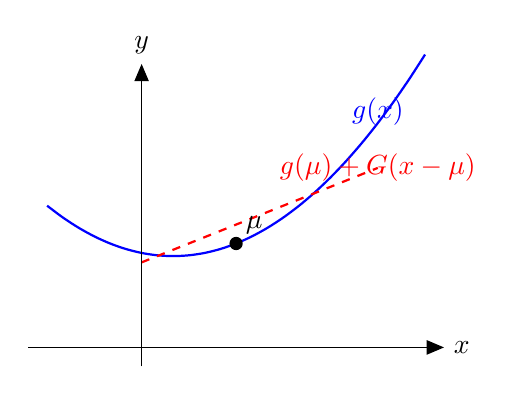
\begin{tikzpicture}[scale=1.2]
    % Nonlinear curve
    \draw[thick, blue] plot[smooth, domain=-1:3] (\x, {0.3*\x*\x - 0.2*\x + 1});

    % Tangent line
    \draw[thick, red, dashed] plot[domain=0:2.5] (\x, {0.4*\x + 0.9});

    % Point of linearization
    \fill (1, 1.1) circle (2pt) node[above right] {$\mu$};

    % Labels
    \node[blue] at (2.5, 2.5) {$g(x)$};
    \node[red] at (2.5, 1.9) {$g(\mu) + G(x-\mu)$};

    % Axes
    \draw[->] (-1.2,0) -- (3.2,0) node[right] {$x$};
    \draw[->] (0,-0.2) -- (0,3) node[above] {$y$};
\end{tikzpicture}
\caption{EKF linearizes nonlinear function around current estimate}
\end{figure}

\subsubsection{The Extended Kalman Filter Algorithm}

\begin{algorithm}[H]
\caption{Extended Kalman Filter}
\KwInput{$\mu_{t-1}$, $\Sigma_{t-1}$, $u_t$, $z_t$}
\KwOutput{$\mu_{t}$, $\Sigma_{t}$}

\BlankLine
\tcp{Compute Jacobian of dynamics}
$G_t = \frac{\partial g}{\partial x}\bigg|_{x=\mu_{t-1}, u=u_t}$\;

\BlankLine
\tcp{Prediction Step}
$\bar{\mu}_t = g(\mu_{t-1}, u_t)$\;
$\bar{\Sigma}_t = G_t \Sigma_{t-1} G_t^T + R_t$\;

\BlankLine
\tcp{Compute Jacobian of measurement model}
$H_t = \frac{\partial h}{\partial x}\bigg|_{x=\bar{\mu}_t}$\;

\BlankLine
\tcp{Kalman Gain}
$K_t = \bar{\Sigma}_t H_t^T (H_t \bar{\Sigma}_t H_t^T + Q_t)^{-1}$\;

\BlankLine
\tcp{Measurement Update}
$\mu_t = \bar{\mu}_t + K_t (z_t - h(\bar{\mu}_t))$\;
$\Sigma_t = (I - K_t H_t)\bar{\Sigma}_t$\;

\BlankLine
\Return{$\mu_{t}$, $\Sigma_{t}$}
\end{algorithm}

\textbf{Differences from KF:}
\begin{enumerate}
    \item Use $g(\mu_{t-1}, u_t)$ instead of $A\mu_{t-1} + Bu_t$
    \item Use $h(\bar{\mu}_t)$ instead of $C\bar{\mu}_t$
    \item Use Jacobians $G_t, H_t$ instead of constant matrices $A, C$
    \item Jacobians must be recomputed each timestep at current estimate
\end{enumerate}

\subsubsection{When Does EKF Work Well?}

\textbf{EKF approximation quality depends on:}

\begin{enumerate}
\item \textbf{Degree of nonlinearity:}
\begin{itemize}
    \item Small nonlinearity $\Rightarrow$ linear approximation good
    \item High nonlinearity $\Rightarrow$ approximation degrades
\end{itemize}

\item \textbf{Uncertainty magnitude:}
\begin{itemize}
    \item Small $\Sigma$ $\Rightarrow$ stay near linearization point $\Rightarrow$ good
    \item Large $\Sigma$ $\Rightarrow$ venture far from linearization point $\Rightarrow$ poor
\end{itemize}
\end{enumerate}

\textbf{Failure modes:}
\begin{itemize}
    \item Highly nonlinear systems with large uncertainty
    \item Linearization point far from true state
    \item Can lead to divergence or inconsistent estimates
\end{itemize}

% ============================================================================
\subsection{Unscented Kalman Filter (UKF)}
% ============================================================================

\subsubsection{Motivation}

\textbf{Problem with EKF:} Linearization can introduce significant errors, especially for highly nonlinear systems.

\textbf{UKF Key Idea:} Instead of linearizing functions, deterministically sample points (sigma points) around the mean, propagate them through the nonlinear function, then compute statistics.

\textbf{Philosophy:} "It's easier to approximate a probability distribution than to approximate an arbitrary nonlinear function."

\subsubsection{The Unscented Transform}

For state dimension $n$, generate $2n+1$ \textbf{sigma points}:
\begin{align}
\mathcal{X}^{[0]} &= \mu \\
\mathcal{X}^{[i]} &= \mu + \left(\sqrt{(n+\lambda)\Sigma}\right)_i, \quad i = 1, \ldots, n \\
\mathcal{X}^{[i]} &= \mu - \left(\sqrt{(n+\lambda)\Sigma}\right)_{i-n}, \quad i = n+1, \ldots, 2n
\end{align}

where $\lambda = \alpha^2(n + \kappa) - n$ is a scaling parameter and $\left(\sqrt{\Sigma}\right)_i$ is the $i$-th column of the matrix square root.

\textbf{Weights:}
\begin{align}
w_m^{[0]} &= \frac{\lambda}{n + \lambda} \\
w_c^{[0]} &= \frac{\lambda}{n + \lambda} + (1 - \alpha^2 + \beta) \\
w_m^{[i]} = w_c^{[i]} &= \frac{1}{2(n + \lambda)}, \quad i = 1, \ldots, 2n
\end{align}

Typical values: $\alpha = 10^{-3}$, $\beta = 2$ (optimal for Gaussian), $\kappa = 0$ or $3-n$.

\subsubsection{UKF Algorithm}

\begin{algorithm}[H]
\caption{Unscented Kalman Filter}
\KwInput{$\mu_{t-1}$, $\Sigma_{t-1}$, $u_t$, $z_t$}
\KwOutput{$\mu_{t}$, $\Sigma_{t}$}

\BlankLine
\tcp{Generate sigma points}
$\lambda = \alpha^2(n+\kappa) - n$\;
$\mathcal{X}_{t-1} = [\mu_{t-1} \quad \mu_{t-1} + \gamma\sqrt{\Sigma_{t-1}} \quad \mu_{t-1} - \gamma\sqrt{\Sigma_{t-1}}]$ where $\gamma = \sqrt{n + \lambda}$\;

\BlankLine
\tcp{Prediction: Propagate sigma points through dynamics}
\For{$i = 0$ to $2n$}{
    $\mathcal{X}_{t|t-1}^{[i]} = g(\mathcal{X}_{t-1}^{[i]}, u_t)$\;
}

\BlankLine
\tcp{Predict mean and covariance}
$\bar{\mu}_t = \sum_{i=0}^{2n} w_m^{[i]} \mathcal{X}_{t|t-1}^{[i]}$\;
$\bar{\Sigma}_t = \sum_{i=0}^{2n} w_c^{[i]} (\mathcal{X}_{t|t-1}^{[i]} - \bar{\mu}_t)(\mathcal{X}_{t|t-1}^{[i]} - \bar{\mu}_t)^T + R_t$\;

\BlankLine
\tcp{Regenerate sigma points from prediction}
$\bar{\mathcal{X}}_t = [\bar{\mu}_t \quad \bar{\mu}_t + \gamma\sqrt{\bar{\Sigma}_t} \quad \bar{\mu}_t - \gamma\sqrt{\bar{\Sigma}_t}]$\;

\BlankLine
\tcp{Propagate through measurement model}
\For{$i = 0$ to $2n$}{
    $\mathcal{Z}_t^{[i]} = h(\bar{\mathcal{X}}_t^{[i]})$\;
}

\BlankLine
\tcp{Predicted measurement statistics}
$\hat{z}_t = \sum_{i=0}^{2n} w_m^{[i]} \mathcal{Z}_t^{[i]}$\;
$S_t = \sum_{i=0}^{2n} w_c^{[i]} (\mathcal{Z}_t^{[i]} - \hat{z}_t)(\mathcal{Z}_t^{[i]} - \hat{z}_t)^T + Q_t$\;
$\bar{\Sigma}_t^{x,z} = \sum_{i=0}^{2n} w_c^{[i]} (\bar{\mathcal{X}}_t^{[i]} - \bar{\mu}_t)(\mathcal{Z}_t^{[i]} - \hat{z}_t)^T$\;

\BlankLine
\tcp{Kalman gain and update}
$K_t = \bar{\Sigma}_t^{x,z} S_t^{-1}$\;
$\mu_t = \bar{\mu}_t + K_t(z_t - \hat{z}_t)$\;
$\Sigma_t = \bar{\Sigma}_t - K_t S_t K_t^T$\;

\BlankLine
\Return{$\mu_{t}$, $\Sigma_{t}$}
\end{algorithm}

\subsubsection{UKF vs EKF}

\begin{tabular}{|l|l|l|}
\hline
\textbf{Property} & \textbf{EKF} & \textbf{UKF} \\
\hline
Jacobian computation & Required & Not needed \\
Accuracy (nonlinear) & First-order approx. & Second-order approx. \\
Computational cost & Lower & Moderate \\
Implementation & Simpler & More complex \\
Divergence risk & Higher & Lower \\
\hline
\end{tabular}

\vspace{3mm}
\textbf{When to use UKF:}
\begin{itemize}
    \item High nonlinearity
    \item Difficult to compute Jacobians
    \item Better accuracy needed
    \item Distribution approximately Gaussian
\end{itemize}

% ============================================================================
\section{Exam Tips \& Common Mistakes}
% ============================================================================

\begin{tcolorbox}[colback=red!10!white,colframe=red!75!black,title=\textbf{Common Exam Mistakes}]

\textbf{1. Jacobian Indexing:}
\begin{itemize}
    \item Remember: row = output equation, column = state variable
    \item Double-check dimensions: $G$ should be $n \times n$ for $n$ states
\end{itemize}

\textbf{2. Evaluation Point:}
\begin{itemize}
    \item $G_t$ evaluated at $\mu_{t-1}$ (before prediction)
    \item $H_t$ evaluated at $\bar{\mu}_t$ (after prediction)
\end{itemize}

\textbf{3. Discretization:}
\begin{itemize}
    \item Don't forget $\Delta t$ when discretizing!
    \item Euler: $x_t = x_{t-1} + \dot{x}_{t-1} \Delta t$
\end{itemize}

\textbf{4. Process Noise Location:}
\begin{itemize}
    \item $R_t$ adds to predicted covariance: $\bar{\Sigma}_t = G\Sigma G^T + R_t$
    \item $Q_t$ adds in Kalman gain: $(H\bar{\Sigma}H^T + Q_t)^{-1}$
\end{itemize}

\textbf{5. Innovation:}
\begin{itemize}
    \item $(z_t - h(\bar{\mu}_t))$ not $(z_t - \bar{\mu}_t)$
    \item Must pass prediction through measurement model!
\end{itemize}

\end{tcolorbox}

% ============================================================================
% END OF KALMAN FILTER NOTES
% ============================================================================

\newpage
% ============================================================================
% ROBOT MOTION - EXAM NOTES
% Focus: Motion models (velocity & odometry), noise parameters
% ============================================================================

\section{Quick Reference: Robot Motion Models}

\begin{tcolorbox}[colback=yellow!10!white,colframe=orange!75!black,title=\textbf{Robot Motion Models - Fast Reference}]

\textbf{Pose Representation:} $x = \begin{bmatrix} x \\ y \\ \theta \end{bmatrix}$ (position + orientation)

\vspace{3mm}
\textbf{Two Motion Models:}

\begin{tabular}{|l|l|l|}
\hline
\textbf{Aspect} & \textbf{Velocity Model} & \textbf{Odometry Model} \\
\hline
Input $u_t$ & $(v_t, \omega_t)$ - commanded velocities & $(\bar{x}_{t-1}, \bar{x}_t)$ - poses from encoders \\
Accuracy & Less accurate & More accurate \\
Availability & Before motion (predictive) & After motion (retrospective) \\
Use case & Motion planning & State estimation \\
\hline
\end{tabular}

\vspace{3mm}
\textbf{Velocity Motion Model:}
\begin{align*}
u_t &= \begin{bmatrix} v \\ \omega \end{bmatrix}, \quad r = \left|\frac{v}{\omega}\right| \quad \text{(circular motion radius)} \\
x_t &= x_{t-1} + \begin{bmatrix}
-\frac{\hat{v}}{\hat{\omega}}\sin\theta + \frac{\hat{v}}{\hat{\omega}}\sin(\theta + \hat{\omega}\Delta t) \\
\frac{\hat{v}}{\hat{\omega}}\cos\theta - \frac{\hat{v}}{\hat{\omega}}\cos(\theta + \hat{\omega}\Delta t) \\
\hat{\omega}\Delta t
\end{bmatrix}
\end{align*}
where $\hat{v} = v + \epsilon_{\alpha_1 v^2 + \alpha_2 \omega^2}$, $\hat{\omega} = \omega + \epsilon_{\alpha_3 v^2 + \alpha_4 \omega^2}$

\vspace{3mm}
\textbf{Odometry Motion Model Decomposition:}
\begin{itemize}
    \item Rotation 1: $\delta_{rot1} = \arctan2(\bar{y}' - \bar{y}, \bar{x}' - \bar{x}) - \bar{\theta}$
    \item Translation: $\delta_{trans} = \sqrt{(\bar{x}' - \bar{x})^2 + (\bar{y}' - \bar{y})^2}$
    \item Rotation 2: $\delta_{rot2} = \bar{\theta}' - \bar{\theta} - \delta_{rot1}$
\end{itemize}

\vspace{3mm}
\textbf{Noise Parameters:}
\begin{itemize}
    \item Velocity: $\alpha_1, \alpha_2$ affect translation, $\alpha_3, \alpha_4$ affect rotation
    \item Odometry: $\alpha_1, \alpha_2$ affect rotations, $\alpha_3, \alpha_4$ affect translation
    \item Larger $\alpha$ = more uncertainty
\end{itemize}

\vspace{3mm}
\textbf{Probability Function:}
$$\text{prob}(a, b^2) = \frac{1}{\sqrt{2\pi b^2}} \exp\left\{-\frac{a^2}{2b^2}\right\} = \mathcal{N}(a; 0, b^2)$$

\end{tcolorbox}

% ============================================================================
\section{Robot Kinematics and Pose}
% ============================================================================

\subsection{Kinematic Configuration}

\textbf{Kinematics} describes how control actions affect robot configuration.

\textbf{For planar mobile robots:}
\begin{itemize}
    \item \textbf{Pose:} $x = \begin{bmatrix} x & y & \theta \end{bmatrix}^T$
    \begin{itemize}
        \item $(x, y)$ - 2D position in global frame
        \item $\theta$ - orientation (heading/bearing) relative to x-axis
    \end{itemize}
    \item \textbf{Location:} Pose without orientation = $(x, y)$
\end{itemize}

\begin{figure}[H]
  \begin{center}
    \includegraphics[width=0.4\textwidth]{images/robot_pose.png}
  \end{center}
  \caption{Robot pose in global coordinate system}
\end{figure}

\subsection{Probabilistic Motion Model}

The \textbf{motion model} specifies the state transition probability:
\begin{equation}
p(x_t \mid u_t, x_{t-1})
\end{equation}

This describes the probability distribution over poses $x_t$ that result from:
\begin{itemize}
    \item Starting at pose $x_{t-1}$
    \item Executing control $u_t$
\end{itemize}

\textbf{Key Insight:} Robot motion is inherently uncertain due to:
\begin{itemize}
    \item Wheel slippage
    \item Uneven terrain
    \item Control inaccuracies
    \item Systematic errors
\end{itemize}

% ============================================================================
\section{Velocity Motion Model}
% ============================================================================

\subsection{Overview}

\textbf{Control input:} $u_t = \begin{bmatrix} v_t \\ \omega_t \end{bmatrix}$
\begin{itemize}
    \item $v_t$ - translational (linear) velocity [m/s]
    \item $\omega_t$ - rotational (angular) velocity [rad/s]
    \item Positive $v$ = forward, positive $\omega$ = counterclockwise
\end{itemize}

\textbf{Use case:} When you have velocity commands (motion planning, prediction)

\subsection{Exact Kinematics (No Noise)}

For constant velocities $(v, \omega)$ over time interval $\Delta t$:

\textbf{Motion on a circle:}
\begin{equation}
r = \left|\frac{v}{\omega}\right| \quad \text{(radius of circular trajectory)}
\end{equation}

Special case: $\omega = 0 \Rightarrow r = \infty$ (straight line)

\textbf{Circle center:} Starting from $x_{t-1} = (x, y, \theta)^T$:
\begin{align}
x_c &= x - \frac{v}{\omega}\sin\theta \\
y_c &= y + \frac{v}{\omega}\cos\theta
\end{align}

\textbf{Final pose after $\Delta t$:}
\begin{equation}
\boxed{
\begin{bmatrix} x' \\ y' \\ \theta' \end{bmatrix} =
\begin{bmatrix} x \\ y \\ \theta \end{bmatrix} +
\begin{bmatrix}
-\frac{v}{\omega}\sin\theta + \frac{v}{\omega}\sin(\theta + \omega\Delta t) \\
\frac{v}{\omega}\cos\theta - \frac{v}{\omega}\cos(\theta + \omega\Delta t) \\
\omega\Delta t
\end{bmatrix}
}
\label{eq:ideal_velocity_motion}
\end{equation}

\begin{figure}[H]
\centering
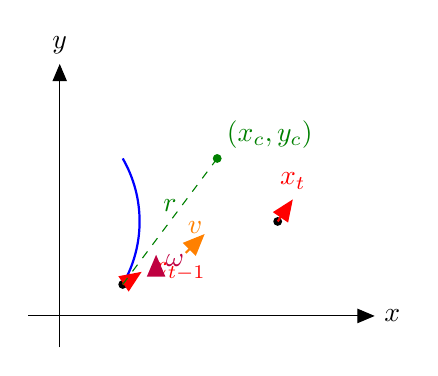
\begin{tikzpicture}[scale=0.8]
    % Draw coordinate system
    \draw[->] (-0.5,0) -- (5,0) node[right] {$x$};
    \draw[->] (0,-0.5) -- (0,4) node[above] {$y$};

    % Draw circular arc
    \draw[thick, blue] (1,0.5) arc (-30:30:2);

    % Start pose
    \fill (1,0.5) circle (2pt);
    \draw[->, thick, red] (1,0.5) -- (1.3,0.7) node[anchor=west] {$x_{t-1}$};

    % End pose
    \fill (3.46,1.5) circle (2pt);
    \draw[->, thick, red] (3.46,1.5) -- (3.7,1.85) node[anchor=south] {$x_t$};

    % Center
    \fill[green!50!black] (2.5,2.5) circle (2pt) node[above right] {$(x_c, y_c)$};
    \draw[dashed, green!50!black] (2.5,2.5) -- (1,0.5) node[midway, above] {$r$};

    % Velocity arrows
    \draw[->, thick, purple] (1.5,0.8) arc (-20:0:0.5) node[midway, right] {$\omega$};
    \draw[->, thick, orange] (2,1) -- (2.3,1.3) node[midway, above] {$v$};

\end{tikzpicture}
\caption{Velocity motion model: robot follows circular arc}
\end{figure}

\subsection{Probabilistic Velocity Model (With Noise)}

Real robots have errors in executing velocity commands.

\textbf{Noise model:} Actual velocities differ from commanded:
\begin{align}
\hat{v} &= v + \epsilon_{\alpha_1 v^2 + \alpha_2 \omega^2} \\
\hat{\omega} &= \omega + \epsilon_{\alpha_3 v^2 + \alpha_4 \omega^2} \\
\hat{\gamma} &= \epsilon_{\alpha_5 v^2 + \alpha_6 \omega^2} \quad \text{(drift)}
\end{align}

where $\epsilon_{b^2}$ denotes a zero-mean Gaussian with variance $b^2$.

\textbf{Noise characteristics:}
\begin{itemize}
    \item Error magnitude proportional to velocity magnitudes
    \item $\alpha_1, \alpha_2$ - translational velocity error parameters
    \item $\alpha_3, \alpha_4$ - rotational velocity error parameters
    \item $\alpha_5, \alpha_6$ - drift error parameters
\end{itemize}

\subsection{Velocity Motion Model Algorithm}

\begin{algorithm}[H]
\caption{Velocity Motion Model: $p(x_t \mid u_t, x_{t-1})$}
\KwInput{$x_t = (x', y', \theta')^T$, $u_t = (v, \omega)^T$, $x_{t-1} = (x, y, \theta)^T$}
\KwOutput{Probability $p(x_t \mid u_t, x_{t-1})$}
\BlankLine
\tcp{Compute ideal (noise-free) control to reach $x_t$ from $x_{t-1}$}
\BlankLine
$\mu = \frac{1}{2}\left[\frac{(x - x')\cos \theta + (y - y') \sin \theta}{(y - y') \cos \theta - (x - x')\sin \theta}\right]$\;
\BlankLine
$x^* = \frac{x+x'}{2} + \mu (y-y')$\;
\BlankLine
$y^* = \frac{y+y'}{2} + \mu (x'-x)$\;
\BlankLine
$r^* = \sqrt{(x-x^*)^2 + (y-y^*)^2}$\;
\BlankLine
$\Delta \theta = \atantwo(y' - y^*,x'-x^*)- \atantwo(y-y^*, x-x^*)$\;
\BlankLine
$\hat{v} = \frac{\Delta \theta}{\dt} r^*$\;
\BlankLine
$\hat{\omega} = \frac{\Delta \theta}{\Delta t}$\;
\BlankLine
$\hat{\gamma} = \frac{\theta' - \theta}{\Delta t} - \hat{\omega}$\;

\BlankLine
\tcp{Compute probability based on difference from commanded velocities}
$p_1 = \text{prob}(v - \hat{v}, \alpha_1 v^2 + \alpha_2 \omega^2)$\;
$p_2 = \text{prob}(\omega - \hat{\omega}, \alpha_3 v^2 + \alpha_4 \omega^2)$\;
$p_3 = \text{prob}(\hat{\gamma}, \alpha_5 v^2 + \alpha_6 \omega^2)$\;

\BlankLine
\Return{$p_1 \cdot p_2 \cdot p_3$}
\end{algorithm}

\textbf{Intuition:}
\begin{enumerate}
    \item Given: start pose $x_{t-1}$, commanded $(v, \omega)$, hypothesized end pose $x_t$
    \item Compute: what velocities $(\hat{v}, \hat{\omega}, \hat{\gamma})$ would be needed to reach $x_t$?
    \item Return: probability that commanded velocities resulted in needed velocities
\end{enumerate}

\begin{figure}[H]
  \begin{center}
    \includegraphics[width=0.6\textwidth]{images/vel_motion_model_noise.png}
  \end{center}
  \caption{Velocity motion model for different noise parameters: (a) moderate noise, (b) large translational noise, (c) large rotational noise}
\end{figure}

% ============================================================================
\section{Odometry Motion Model}
% ============================================================================

\subsection{Overview}

\textbf{Control input:} $u_t = \begin{bmatrix} \bar{x}_{t-1} \\ \bar{x}_t \end{bmatrix}$ where $\bar{x} = (\bar{x}, \bar{y}, \bar{\theta})^T$
\begin{itemize}
    \item $\bar{x}_{t-1}$, $\bar{x}_t$ - poses from robot's internal odometry (wheel encoders)
    \item Bar notation indicates odometry frame (not global frame)
\end{itemize}

\textbf{Key idea:}
\begin{itemize}
    \item Robot's internal odometry frame doesn't match global frame
    \item But \textit{relative motion} in odometry frame approximates relative motion in global frame
    \item Use odometry readings to estimate motion, not absolute position
\end{itemize}

\textbf{Use case:} State estimation after motion has occurred (more accurate than velocity model)

\textbf{Why more accurate?}
\begin{itemize}
    \item Measures actual wheel rotations (not just commands)
    \item No model mismatch between commanded and achieved velocities
    \item Still suffers from drift and slippage (but less than velocity model)
\end{itemize}

\subsection{Odometry Decomposition}

Any planar motion can be decomposed into: \textbf{Rotate → Translate → Rotate}

\begin{figure}[H]
  \begin{center}
    \includegraphics[width=0.45\textwidth]{images/odom_model.png}
  \end{center}
  \caption{Odometry motion decomposition into three steps}
\end{figure}

\begin{tcolorbox}[colback=blue!5!white,colframe=blue!75!black,title=Odometry Decomposition Formulas]

Given odometry readings $\bar{x}_{t-1} = (\bar{x}, \bar{y}, \bar{\theta})$ and $\bar{x}_t = (\bar{x}', \bar{y}', \bar{\theta}')$:

\vspace{2mm}
\textbf{Step 1: Initial rotation} (align with direction of translation)
\begin{equation}
\delta_{rot1} = \arctan2(\bar{y}' - \bar{y}, \bar{x}' - \bar{x}) - \bar{\theta}
\end{equation}

\textbf{Step 2: Translation} (straight-line distance)
\begin{equation}
\delta_{trans} = \sqrt{(\bar{x}' - \bar{x})^2 + (\bar{y}' - \bar{y})^2}
\end{equation}

\textbf{Step 3: Final rotation} (achieve final orientation)
\begin{equation}
\delta_{rot2} = \bar{\theta}' - \bar{\theta} - \delta_{rot1}
\end{equation}

\textbf{Important:} All angles must be normalized to $[-\pi, \pi]$

\end{tcolorbox}

\subsection{Probabilistic Odometry Model}

Each of the three motion components ($\delta_{rot1}, \delta_{trans}, \delta_{rot2}$) is corrupted by noise:

\textbf{Noise model:}
\begin{align}
\delta_{rot1} &\rightarrow \delta_{rot1} + \epsilon_{\alpha_1 |\delta_{rot1}| + \alpha_2 \delta_{trans}} \\
\delta_{trans} &\rightarrow \delta_{trans} + \epsilon_{\alpha_3 \delta_{trans} + \alpha_4(|\delta_{rot1}| + |\delta_{rot2}|)} \\
\delta_{rot2} &\rightarrow \delta_{rot2} + \epsilon_{\alpha_1 |\delta_{rot2}| + \alpha_2 \delta_{trans}}
\end{align}

\textbf{Noise parameters:}
\begin{itemize}
    \item $\alpha_1$ - rotation error from rotation
    \item $\alpha_2$ - rotation error from translation
    \item $\alpha_3$ - translation error from translation
    \item $\alpha_4$ - translation error from rotation
\end{itemize}

\subsection{Odometry Motion Model Algorithm}

\begin{algorithm}[H]
\caption{Odometry Motion Model: $p(x_t \mid u_t, x_{t-1})$}
\KwInput{$x_t = (x', y', \theta')^T$, $u_t = (\bar{x}_{t-1}, \bar{x}_t)$, $x_{t-1} = (x, y, \theta)^T$}
\KwOutput{Probability $p(x_t \mid u_t, x_{t-1})$}

\BlankLine
\tcp{Extract relative motion from odometry readings}
$\delta_{rot1} = \arctan2(\bar{y}' - \bar{y}, \bar{x}' - \bar{x}) - \bar{\theta}$\;
$\delta_{trans} = \sqrt{(\bar{x}' - \bar{x})^2 + (\bar{y}' - \bar{y})^2}$\;
$\delta_{rot2} = \bar{\theta}' - \bar{\theta} - \delta_{rot1}$\;

\BlankLine
\tcp{Compute expected motion from true poses}
$\hat{\delta}_{rot1} = \arctan2(y' - y, x' - x) - \theta$\;
$\hat{\delta}_{trans} = \sqrt{(x' - x)^2 + (y' - y)^2}$\;
$\hat{\delta}_{rot2} = \theta' - \theta - \hat{\delta}_{rot1}$\;

\BlankLine
\tcp{Compute probability of each motion component}
$p_1 = \text{prob}(\delta_{rot1} - \hat{\delta}_{rot1}, \alpha_1 \hat{\delta}_{rot1}^2 + \alpha_2 \hat{\delta}_{trans}^2)$\;
$p_2 = \text{prob}(\delta_{trans} - \hat{\delta}_{trans}, \alpha_3 \hat{\delta}_{trans}^2 + \alpha_4 (\hat{\delta}_{rot1}^2 + \hat{\delta}_{rot2}^2))$\;
$p_3 = \text{prob}(\delta_{rot2} - \hat{\delta}_{rot2}, \alpha_1 \hat{\delta}_{rot2}^2 + \alpha_2 \hat{\delta}_{trans}^2)$\;

\BlankLine
\Return{$p_1 \cdot p_2 \cdot p_3$}
\end{algorithm}

\textbf{Intuition:}
\begin{enumerate}
    \item \textbf{From odometry:} Extract what motion the robot \textit{thinks} it did ($\delta$'s)
    \item \textbf{From true poses:} Compute what motion \textit{actually occurred} ($\hat{\delta}$'s)
    \item \textbf{Compare:} Probability based on difference (larger difference = less likely)
\end{enumerate}

\textbf{Critical implementation detail:} Normalize all angular differences to $[-\pi, \pi]$ before computing probabilities!

\begin{figure}[H]
  \begin{center}
    \includegraphics[width=0.65\textwidth]{images/odom_motion_model_noise.png}
  \end{center}
  \caption{Odometry motion model for different noise parameters: (a) typical noise, (b) large translational error, (c) large rotational error}
\end{figure}

% ============================================================================
\section{Comparison: Velocity vs. Odometry Models}
% ============================================================================

\begin{tcolorbox}[colback=green!5!white,colframe=green!60!black,title=Model Comparison]

\begin{tabular}{|l|p{5cm}|p{5cm}|}
\hline
\textbf{Property} & \textbf{Velocity Model} & \textbf{Odometry Model} \\
\hline
\textbf{Input} & Commanded velocities $(v, \omega)$ & Encoder-based poses $(\bar{x}_{t-1}, \bar{x}_t)$ \\
\hline
\textbf{Availability} & Before motion (predictive) & After motion (retrospective) \\
\hline
\textbf{Accuracy} & Lower (model mismatch) & Higher (measures actual motion) \\
\hline
\textbf{Suitable for} & Motion planning, prediction & State estimation, localization \\
\hline
\textbf{Error sources} &
$\bullet$ Control inaccuracy \newline
$\bullet$ Model mismatch \newline
$\bullet$ Slippage \newline
$\bullet$ Drift &
$\bullet$ Slippage \newline
$\bullet$ Drift \newline
$\bullet$ Encoder resolution \\
\hline
\textbf{Noise params} & $\alpha_1$ to $\alpha_6$ & $\alpha_1$ to $\alpha_4$ \\
\hline
\textbf{Update freq} & Low $\Rightarrow$ models differ & High $\Rightarrow$ models similar \\
\hline
\end{tabular}

\vspace{3mm}
\textbf{Rule of thumb:}
\begin{itemize}
    \item High-frequency updates ($\Delta t$ small) $\Rightarrow$ models similar
    \item Low-frequency updates ($\Delta t$ large) $\Rightarrow$ odometry more accurate
\end{itemize}

\end{tcolorbox}

% ============================================================================
\section{Implementation Notes}
% ============================================================================

\subsection{Common Pitfalls and Best Practices}

\begin{tcolorbox}[colback=red!5!white,colframe=red!75!black,title=\textbf{EXAM CRITICAL: Implementation Issues}]

\textbf{1. Angle Wrapping}
\begin{itemize}
    \item Always normalize angles to $[-\pi, \pi]$ or $[0, 2\pi)$
    \item Especially important in odometry model for $\delta_{rot1}$ and $\delta_{rot2}$
    \item Use: \texttt{atan2(y, x)} not \texttt{atan(y/x)} (handles quadrants correctly)
\end{itemize}

\textbf{2. Division by Zero}
\begin{itemize}
    \item In velocity model: $\omega = 0 \Rightarrow$ straight line motion
    \item Handle separately: $x' = x + v\cos\theta \cdot \Delta t$, $y' = y + v\sin\theta \cdot \Delta t$
\end{itemize}

\textbf{3. Coordinate Frames}
\begin{itemize}
    \item \textbf{Velocity model:} All in global frame
    \item \textbf{Odometry model:} Extract relative motion (frame-independent), then apply to global poses
\end{itemize}

\textbf{4. Noise Parameters}
\begin{itemize}
    \item Must be determined experimentally for each robot
    \item Larger values = more conservative (spread out distribution)
    \item Different surfaces $\Rightarrow$ different parameters (e.g., carpet vs. tile)
\end{itemize}

\textbf{5. Probability Function}
\begin{itemize}
    \item Can use Gaussian: $\text{prob}(a, b^2) = \frac{1}{\sqrt{2\pi b^2}}\exp\{-\frac{a^2}{2b^2}\}$
    \item Or triangular distribution for computational efficiency
    \item Must integrate/sum to 1 over all hypotheses
\end{itemize}

\end{tcolorbox}

\subsection{Parameter Tuning Guidelines}

\textbf{Velocity model parameters $(\alpha_1, \ldots, \alpha_6)$:}
\begin{itemize}
    \item Start with all $\alpha_i = 0.01$ (1\% error)
    \item Increase $\alpha_1, \alpha_2$ if robot struggles with straight-line accuracy
    \item Increase $\alpha_3, \alpha_4$ if robot struggles with turning accuracy
    \item Increase $\alpha_5, \alpha_6$ if systematic drift observed
\end{itemize}

\textbf{Odometry model parameters $(\alpha_1, \ldots, \alpha_4)$:}
\begin{itemize}
    \item Typical values: $\alpha_1 = 0.001$, $\alpha_2 = 0.001$, $\alpha_3 = 0.01$, $\alpha_4 = 0.01$
    \item Translation often more accurate than rotation
    \item Test on known trajectories (e.g., square, circle) and adjust
\end{itemize}

% ============================================================================
\section{Connection to Lab 4}
% ============================================================================

\begin{tcolorbox}[colback=yellow!5!white,colframe=orange!75!black,title=Your Lab 4 Implementation]

Your Lab 4 EKF uses a \textbf{hybrid approach}:

\vspace{2mm}
\textbf{Dynamics (prediction):}
\begin{itemize}
    \item Velocity-based with first-order model: $v_t = av_{t-1} + (1-a)u_v$
    \item More sophisticated than basic velocity model (includes dynamics)
\end{itemize}

\textbf{Measurements (correction):}
\begin{itemize}
    \item Wheel encoders: directly measure $\omega_r, \omega_l$
    \item IMU gyroscope: directly measure $\omega_g$
    \item Related to velocities via kinematics (like odometry uses encoder data)
\end{itemize}

\textbf{Key difference from textbook models:}
\begin{itemize}
    \item Your lab measures velocities directly (encoders + IMU)
    \item Textbook odometry integrates encoders into pose estimates
    \item Your approach: fuses raw sensor data optimally via EKF
\end{itemize}

\end{tcolorbox}

% ============================================================================
\section{Exam Preparation Summary}
% ============================================================================

\begin{tcolorbox}[colback=red!10!white,colframe=red!75!black,title=\textbf{What to Memorize for Exam}]

\textbf{1. Key Formulas:}
\begin{itemize}
    \item Velocity model: circular motion radius $r = |v/\omega|$
    \item Odometry decomposition: $\delta_{rot1}$, $\delta_{trans}$, $\delta_{rot2}$
    \item Noise model: variance proportional to squared velocities/motions
\end{itemize}

\textbf{2. When to Use Which Model:}
\begin{itemize}
    \item Velocity: planning (before motion)
    \item Odometry: estimation (after motion)
\end{itemize}

\textbf{3. Algorithm Structure:}
\begin{itemize}
    \item Both: compute ideal motion $\rightarrow$ compare to actual $\rightarrow$ return probability
    \item Independence assumption: $p_{total} = p_1 \cdot p_2 \cdot p_3$
\end{itemize}

\textbf{4. Implementation Issues:}
\begin{itemize}
    \item Angle normalization (critical!)
    \item Division by zero in velocity model
    \item \texttt{atan2} vs \texttt{atan}
\end{itemize}

\textbf{5. Noise Parameters:}
\begin{itemize}
    \item Know what each $\alpha_i$ represents
    \item Larger values = more uncertainty in that component
\end{itemize}

\end{tcolorbox}

% ============================================================================
% END OF ROBOT MOTION NOTES
% ============================================================================

\newpage
% ============================================================================
% ROBOT LOCALIZATION - EXAM NOTES
% Focus: EKF localization, feature-based maps, data association
% ============================================================================

\section{Quick Reference: EKF Localization}

\begin{tcolorbox}[colback=yellow!10!white,colframe=orange!75!black,title=\textbf{EKF Localization - Fast Reference}]

\textbf{Problem:} Estimate robot pose $x = [x, y, \theta]^T$ given:
\begin{itemize}
    \item Map $m$ with known landmark locations
    \item Motion commands $u_t = [v_t, \omega_t]^T$
    \item Sensor measurements $z_t = \{z_t^1, z_t^2, \ldots\}$ to landmarks
\end{itemize}

\vspace{3mm}
\textbf{Measurement Model (Range-Bearing):}
\begin{equation*}
z_t^i = \begin{bmatrix} r_t^i \\ \phi_t^i \\ s_t^i \end{bmatrix} = 
\begin{bmatrix} 
\sqrt{(m_{j,x} - x)^2 + (m_{j,y} - y)^2} \\ 
\arctan2(m_{j,y} - y, m_{j,x} - x) - \theta \\ 
m_{j,s} 
\end{bmatrix} + \text{noise}
\end{equation*}
where $r$ = range, $\phi$ = bearing, $s$ = signature (landmark ID feature)

\vspace{3mm}
\textbf{Measurement Jacobian $H_t$:} (Evaluated at $\bar{\mu}_t$)
\begin{equation*}
H_t^i = \begin{bmatrix} 
-\frac{\Delta x}{\sqrt{q}} & -\frac{\Delta y}{\sqrt{q}} & 0 \\[3pt]
\frac{\Delta y}{q} & -\frac{\Delta x}{q} & -1 \\[3pt]
0 & 0 & 0 
\end{bmatrix}
\end{equation*}
where $\Delta x = m_{j,x} - \bar{\mu}_{t,x}$, $\Delta y = m_{j,y} - \bar{\mu}_{t,y}$, $q = \Delta x^2 + \Delta y^2$

\vspace{3mm}
\textbf{Key Difference: Motion Model Jacobian}
\begin{itemize}
    \item $G_t$ - Jacobian of motion w.r.t. \textbf{pose} (like Lab 4)
    \item $V_t$ - Jacobian of motion w.r.t. \textbf{control} (new!)
    \item Process noise: $\bar{\Sigma}_t = G_t \Sigma_{t-1} G_t^T + V_t M_t V_t^T$
\end{itemize}

\vspace{3mm}
\textbf{Two Versions:}
\begin{enumerate}
    \item \textbf{Known correspondences:} If you know which landmark you're observing
    \item \textbf{Unknown correspondences:} Must do data association (find $\arg\max$ likelihood)
\end{enumerate}

\end{tcolorbox}

% ============================================================================
\section{The Localization Problem}
% ============================================================================

\subsection{Problem Definition}

\textbf{Localization:} Determine robot's pose $x_t = [x, y, \theta]^T$ relative to a known map $m$.

\begin{itemize}
    \item Also called \textbf{position estimation}
    \item Fundamental problem in robotics
    \item Establishes correspondence between map frame and robot's local frame
\end{itemize}

\textbf{Why is it hard?}
\begin{itemize}
    \item Pose cannot be sensed directly
    \item Single measurement usually insufficient
    \item Must integrate noisy data over time
    \item Uncertainty from both motion and sensors
\end{itemize}

\begin{figure}[H]
\centering
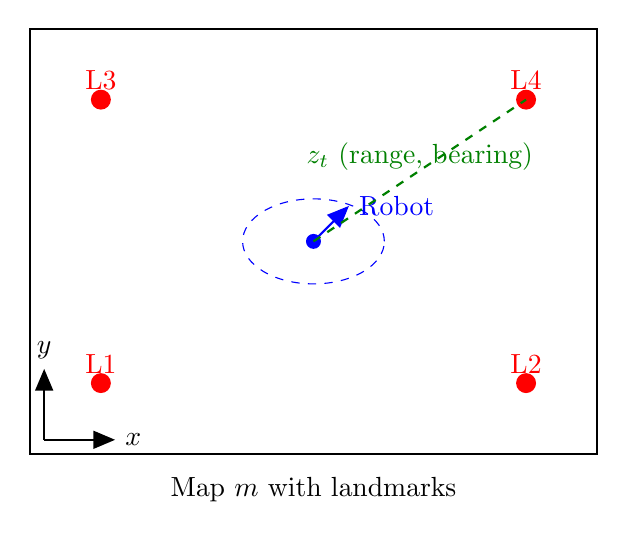
\begin{tikzpicture}[scale=0.9]
    % Draw map with landmarks
    \draw[thick] (0,0) rectangle (8,6);
    
    % Landmarks
    \foreach \x/\y/\label in {1/1/L1, 7/1/L2, 1/5/L3, 7/5/L4} {
        \fill[red] (\x,\y) circle (4pt);
        \node[red, above] at (\x,\y) {\label};
    }
    
    % Robot (with uncertainty ellipse)
    \fill[blue] (4,3) circle (3pt);
    \draw[->, thick, blue] (4,3) -- (4.5,3.5) node[right] {Robot};
    \draw[blue, dashed] (4,3) ellipse (1cm and 0.6cm);
    
    % Measurement to landmark
    \draw[green!50!black, thick, dashed] (4,3) -- (7,5);
    \node[green!50!black] at (5.5,4.2) {$z_t$ (range, bearing)};
    
    % Coordinate frame
    \draw[->, thick] (0.2,0.2) -- (1.2,0.2) node[right] {$x$};
    \draw[->, thick] (0.2,0.2) -- (0.2,1.2) node[above] {$y$};
    
    \node at (4,-0.5) {Map $m$ with landmarks};
\end{tikzpicture}
\caption{Localization: estimate robot pose given map and measurements to landmarks}
\end{figure}

\subsection{Three Types of Localization Problems}

\begin{tcolorbox}[colback=blue!5!white,colframe=blue!75!black,title=Localization Problem Types]

\textbf{1. Position Tracking}
\begin{itemize}
    \item Initial pose is \textbf{known}
    \item Track small deviations over time
    \item Initial belief: $bel(x_0) = \delta(\bar{x}_0)$ (point-mass at known pose)
    \item \textbf{Easier problem} - local, unimodal
\end{itemize}

\textbf{2. Global Localization}
\begin{itemize}
    \item Initial pose is \textbf{unknown}
    \item Must determine pose from scratch
    \item Initial belief: $bel(x_0) = \frac{1}{|X|}$ (uniform over all valid poses)
    \item \textbf{Harder problem} - global, potentially multi-modal
\end{itemize}

\textbf{3. Kidnapped Robot Problem}
\begin{itemize}
    \item Robot is "kidnapped" and moved to unknown location during operation
    \item Must detect that localization has failed and re-localize
    \item \textbf{Hardest problem} - requires fault detection
\end{itemize}

\end{tcolorbox}

\textbf{Note:} EKF localization (Gaussian) is best for position tracking. Global localization often requires multi-hypothesis methods (particle filters, grid-based methods).

% ============================================================================
\section{Markov Localization (General Framework)}
% ============================================================================

\textbf{Markov localization} is the direct application of Bayes filter to localization.

\subsection{The Algorithm}

\begin{algorithm}[H]
\caption{Markov Localization}
\KwInput{$bel(x_{t-1})$, $u_t$, $z_t$, map $m$}
\KwOutput{$bel(x_t)$}

\BlankLine
\tcp{Prediction Step}
\For{all $x_t$}{
    $\bar{bel}(x_t) = \int p(x_t \mid u_t, x_{t-1}, m) \cdot bel(x_{t-1}) \, dx_{t-1}$\;
}

\BlankLine
\tcp{Correction Step}
\For{all $x_t$}{
    $bel(x_t) = \eta \cdot p(z_t \mid x_t, m) \cdot \bar{bel}(x_t)$\;
}

\BlankLine
\Return{$bel(x_t)$}
\end{algorithm}

\textbf{Key differences from basic Bayes filter:}
\begin{itemize}
    \item Map $m$ is given and fixed
    \item Motion model: $p(x_t \mid u_t, x_{t-1}, m)$ - may use map (e.g., for collision detection)
    \item Measurement model: $p(z_t \mid x_t, m)$ - compares observation to expected measurement from map
\end{itemize}

% ============================================================================
\section{EKF Localization: Feature-Based Maps}
% ============================================================================

\subsection{Map Representation}

\textbf{Feature-based map:} Collection of point landmarks
\begin{equation}
m = \{m_1, m_2, \ldots, m_N\}
\end{equation}

Each landmark $m_j$ has:
\begin{equation}
m_j = [m_{j,x}, m_{j,y}, m_{j,s}]^T
\end{equation}
where:
\begin{itemize}
    \item $(m_{j,x}, m_{j,y})$ - landmark location in global frame
    \item $m_{j,s}$ - landmark signature (unique identifier or feature descriptor)
\end{itemize}

\subsection{Measurement Model}

At time $t$, robot observes multiple features: $z_t = \{z_t^1, z_t^2, \ldots, z_t^{k_t}\}$

Each measurement $z_t^i$ consists of:
\begin{equation}
z_t^i = \begin{bmatrix} r_t^i \\ \phi_t^i \\ s_t^i \end{bmatrix}
\end{equation}

\begin{itemize}
    \item $r_t^i$ - \textbf{range} (distance) to landmark
    \item $\phi_t^i$ - \textbf{bearing} (angle) to landmark relative to robot heading
    \item $s_t^i$ - \textbf{signature} of landmark (what type/ID it is)
\end{itemize}

\begin{figure}[H]
\centering
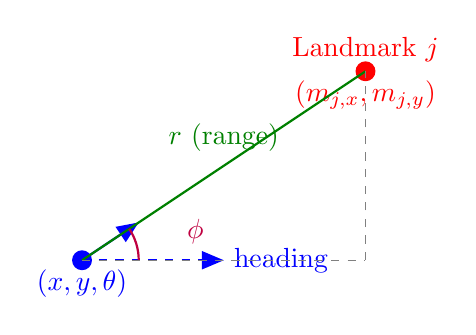
\begin{tikzpicture}[scale=1.2]
    % Robot
    \fill[blue] (2,2) circle (3pt);
    \draw[->, thick, blue] (2,2) -- (2.6,2.4);
    \node[blue, below] at (2,2) {$(x, y, \theta)$};
    
    % Robot heading
    \draw[->, thick, blue, dashed] (2,2) -- (3.5,2) node[right] {heading};
    
    % Landmark
    \fill[red] (5,4) circle (3pt);
    \node[red, above] at (5,4) {Landmark $j$};
    \node[red, below] at (5,4) {$(m_{j,x}, m_{j,y})$};
    
    % Range
    \draw[green!50!black, thick] (2,2) -- (5,4);
    \node[green!50!black] at (3.5,3.3) {$r$ (range)};
    
    % Bearing angle
    \draw[purple, thick] (2.6,2) arc (0:33.7:0.6);
    \node[purple] at (3.2,2.3) {$\phi$};
    
    % Angle measurement
    \draw[gray, dashed] (2,2) -- (5,2);
    \draw[gray, dashed] (5,2) -- (5,4);
\end{tikzpicture}
\caption{Range-bearing measurement model}
\end{figure}

\subsection{Expected Measurement Function}

Given robot pose $x = [x, y, \theta]^T$ and landmark $m_j$, expected measurement is:

\begin{equation}
\boxed{
h(x, m_j) = \begin{bmatrix} 
\sqrt{(m_{j,x} - x)^2 + (m_{j,y} - y)^2} \\[5pt]
\arctan2(m_{j,y} - y, m_{j,x} - x) - \theta \\[5pt]
m_{j,s} 
\end{bmatrix}
}
\label{eq:measurement_function}
\end{equation}

Let $\Delta x = m_{j,x} - x$, $\Delta y = m_{j,y} - y$, and $q = \Delta x^2 + \Delta y^2$. Then:

\begin{equation}
h(x, m_j) = \begin{bmatrix} \sqrt{q} \\ \arctan2(\Delta y, \Delta x) - \theta \\ m_{j,s} \end{bmatrix}
\end{equation}

\textbf{Actual measurement:} $z_t^i = h(x_t, m_j) + \epsilon$ where $\epsilon \sim \mathcal{N}(0, Q_t)$

\subsection{Measurement Jacobian}

To linearize for EKF, compute Jacobian w.r.t. robot pose:

\begin{equation}
H_t^i = \frac{\partial h}{\partial x}\bigg|_{x=\bar{\mu}_t} = 
\boxed{
\begin{bmatrix} 
-\frac{\Delta x}{\sqrt{q}} & -\frac{\Delta y}{\sqrt{q}} & 0 \\[5pt]
\frac{\Delta y}{q} & -\frac{\Delta x}{q} & -1 \\[5pt]
0 & 0 & 0 
\end{bmatrix}
}
\label{eq:measurement_jacobian}
\end{equation}

where all quantities evaluated at predicted pose $\bar{\mu}_t$:
\begin{align}
\Delta x &= m_{j,x} - \bar{\mu}_{t,x} \\
\Delta y &= m_{j,y} - \bar{\mu}_{t,y} \\
q &= \Delta x^2 + \Delta y^2
\end{align}

\textbf{Derivation notes:}
\begin{itemize}
    \item Row 1: $\frac{\partial}{\partial x}[\sqrt{q}] = \frac{1}{2\sqrt{q}} \cdot 2\Delta x \cdot (-1) = -\frac{\Delta x}{\sqrt{q}}$
    \item Row 2: $\frac{\partial}{\partial x}[\arctan2(\Delta y, \Delta x)] = \frac{\Delta y}{q}$ (chain rule on atan)
    \item Row 3: Signature doesn't depend on robot pose
\end{itemize}

\begin{tcolorbox}[colback=green!5!white,colframe=green!60!black,title=Understanding the Jacobian]

\textbf{Physical interpretation of $H_t$:}

\begin{itemize}
    \item \textbf{Row 1:} How range $r$ changes with small pose changes
    \begin{itemize}
        \item Moving toward landmark ($+\Delta x$ if landmark is to the right) decreases range
        \item Hence negative sign
    \end{itemize}
    
    \item \textbf{Row 2:} How bearing $\phi$ changes with small pose changes
    \begin{itemize}
        \item Moving perpendicular to line-of-sight changes bearing most
        \item Robot rotation directly affects bearing (hence $-1$ in $\theta$ column)
    \end{itemize}
    
    \item \textbf{Row 3:} Signature independent of pose (all zeros)
\end{itemize}

\end{tcolorbox}

% ============================================================================
\section{Motion Model for Localization}
% ============================================================================

EKF localization typically uses the \textbf{velocity motion model}:

\begin{equation}
x_t = x_{t-1} + \begin{bmatrix}
-\frac{v_t}{\omega_t}\sin\theta + \frac{v_t}{\omega_t}\sin(\theta + \omega_t\Delta t) \\
\frac{v_t}{\omega_t}\cos\theta - \frac{v_t}{\omega_t}\cos(\theta + \omega_t\Delta t) \\
\omega_t\Delta t
\end{bmatrix} + \epsilon
\end{equation}

\subsection{Two Jacobians for Motion Model}

\textbf{1. Jacobian w.r.t. state $G_t$:} (Like Lab 4)
\begin{equation}
G_t = \frac{\partial g}{\partial x}\bigg|_{x=\mu_{t-1}} = 
\begin{bmatrix} 
1 & 0 & -\frac{v_t}{\omega_t}\cos\theta + \frac{v_t}{\omega_t}\cos(\theta + \omega_t\Delta t) \\
0 & 1 & -\frac{v_t}{\omega_t}\sin\theta + \frac{v_t}{\omega_t}\sin(\theta + \omega_t\Delta t) \\
0 & 0 & 1 
\end{bmatrix}
\end{equation}

\textbf{2. Jacobian w.r.t. control $V_t$:} (New for localization!)
\begin{equation}
V_t = \frac{\partial g}{\partial u}\bigg|_{u=u_t} = 
\begin{bmatrix}
\frac{-\sin\theta + \sin(\theta+\omega_t\Delta t)}{\omega_t} & \frac{v_t(\sin\theta - \sin(\theta+\omega_t\Delta t))}{\omega_t^2} + \frac{v_t\cos(\theta+\omega_t\Delta t)\Delta t}{\omega_t} \\
\frac{\cos\theta - \cos(\theta+\omega_t\Delta t)}{\omega_t} & -\frac{v_t(\cos\theta - \cos(\theta+\omega_t\Delta t))}{\omega_t^2} + \frac{v_t\sin(\theta+\omega_t\Delta t)\Delta t}{\omega_t} \\
0 & \Delta t
\end{bmatrix}
\end{equation}

\textbf{Control noise covariance:}
\begin{equation}
M_t = \begin{bmatrix} 
\alpha_1 v_t^2 + \alpha_2 \omega_t^2 & 0 \\ 
0 & \alpha_3 v_t^2 + \alpha_4 \omega_t^2 
\end{bmatrix}
\end{equation}

\textbf{Predicted covariance:}
\begin{equation}
\boxed{\bar{\Sigma}_t = G_t \Sigma_{t-1} G_t^T + V_t M_t V_t^T}
\end{equation}

This accounts for:
\begin{itemize}
    \item Uncertainty propagation from previous pose ($G_t \Sigma_{t-1} G_t^T$)
    \item Control noise ($V_t M_t V_t^T$)
\end{itemize}

% ============================================================================
\section{EKF Localization Algorithm}
% ============================================================================

\subsection{Version 1: Known Correspondences}

\textbf{Assumption:} For each measurement $z_t^i$, we know which landmark $c_t^i = j$ it corresponds to.

\begin{algorithm}[H]
\caption{EKF Localization (Known Correspondences)}
\KwInput{$\mu_{t-1}$, $\Sigma_{t-1}$, $u_t$, $z_t$, $c_t$, map $m$}
\KwOutput{$\mu_t$, $\Sigma_t$}

\BlankLine
\tcp{PREDICTION STEP}
Compute $G_t$, $V_t$, $M_t$ from motion model\;
$\bar{\mu}_t = \mu_{t-1} + g(u_t, \mu_{t-1})$ \tcp{predicted mean}
$\bar{\Sigma}_t = G_t \Sigma_{t-1} G_t^T + V_t M_t V_t^T$ \tcp{predicted covariance}

\BlankLine
\tcp{CORRECTION STEP (for each observed feature)}
$Q_t = \text{diag}(\sigma_r^2, \sigma_\phi^2, \sigma_s^2)$ \tcp{measurement noise}

\For{each observed feature $z_t^i = [r_t^i, \phi_t^i, s_t^i]^T$}{
    $j = c_t^i$ \tcp{known correspondence}
    
    \tcp{Compute expected measurement}
    $\Delta x = m_{j,x} - \bar{\mu}_{t,x}$, $\Delta y = m_{j,y} - \bar{\mu}_{t,y}$, $q = \Delta x^2 + \Delta y^2$\;
    $\hat{z}_t^i = \begin{bmatrix} \sqrt{q} \\ \arctan2(\Delta y, \Delta x) - \bar{\mu}_{t,\theta} \\ m_{j,s} \end{bmatrix}$\;
    
    \tcp{Compute measurement Jacobian}
    $H_t^i = \begin{bmatrix} 
    -\frac{\Delta x}{\sqrt{q}} & -\frac{\Delta y}{\sqrt{q}} & 0 \\
    \frac{\Delta y}{q} & -\frac{\Delta x}{q} & -1 \\
    0 & 0 & 0 
    \end{bmatrix}$\;
    
    \tcp{Kalman gain and update}
    $S_t^i = H_t^i \bar{\Sigma}_t [H_t^i]^T + Q_t$ \tcp{innovation covariance}
    $K_t^i = \bar{\Sigma}_t [H_t^i]^T [S_t^i]^{-1}$ \tcp{Kalman gain}
    $\bar{\mu}_t = \bar{\mu}_t + K_t^i (z_t^i - \hat{z}_t^i)$ \tcp{update mean}
    $\bar{\Sigma}_t = (I - K_t^i H_t^i) \bar{\Sigma}_t$ \tcp{update covariance}
}

\BlankLine
$\mu_t = \bar{\mu}_t$, $\Sigma_t = \bar{\Sigma}_t$\;
\Return{$\mu_t$, $\Sigma_t$}
\end{algorithm}

\textbf{Key points:}
\begin{itemize}
    \item Process measurements \textbf{sequentially}
    \item Each measurement refines the belief
    \item After all measurements: $\mu_t$ and $\Sigma_t$ are final estimates
\end{itemize}

% ============================================================================
\subsection{Version 2: Unknown Correspondences (Data Association)}
% ============================================================================

\textbf{Problem:} We don't know which landmark each measurement corresponds to!

\textbf{Solution:} For each measurement, find the landmark that best explains it (maximum likelihood).

\begin{tcolorbox}[colback=red!5!white,colframe=red!75!black,title=The Data Association Problem]

Given measurement $z_t^i$, which landmark $j$ in the map did it come from?

\textbf{Approach:} Test all landmarks, pick most likely:
\begin{equation}
j^*(i) = \arg\max_j \, p(z_t^i \mid \bar{\mu}_t, m_j)
\end{equation}

This is a \textbf{maximum likelihood} correspondence estimator.

\textbf{The likelihood:}
\begin{equation}
p(z_t^i \mid \bar{\mu}_t, m_j) = \det(2\pi S_t^j)^{-1/2} \exp\left\{-\frac{1}{2}(z_t^i - \hat{z}_t^j)^T [S_t^j]^{-1} (z_t^i - \hat{z}_t^j)\right\}
\end{equation}

where $\hat{z}_t^j$ is expected measurement from landmark $j$ and $S_t^j$ is innovation covariance.

\end{tcolorbox}

\begin{algorithm}[H]
\caption{EKF Localization (Unknown Correspondences)}
\KwInput{$\mu_{t-1}$, $\Sigma_{t-1}$, $u_t$, $z_t$, map $m$}
\KwOutput{$\mu_t$, $\Sigma_t$}

\BlankLine
\tcp{PREDICTION STEP (same as before)}
Compute $G_t$, $V_t$, $M_t$\;
$\bar{\mu}_t = \mu_{t-1} + g(u_t, \mu_{t-1})$\;
$\bar{\Sigma}_t = G_t \Sigma_{t-1} G_t^T + V_t M_t V_t^T$\;

\BlankLine
\tcp{CORRECTION WITH DATA ASSOCIATION}
$Q_t = \text{diag}(\sigma_r^2, \sigma_\phi^2, \sigma_s^2)$\;

\For{each observed feature $z_t^i$}{
    \tcp{Test all landmarks to find best match}
    \For{each landmark $k$ in map $m$}{
        Compute $\hat{z}_t^k$, $H_t^k$, $S_t^k$ as before\;
        Compute likelihood $\mathcal{L}_k = \det(2\pi S_t^k)^{-1/2} \exp\{-\frac{1}{2}(z_t^i - \hat{z}_t^k)^T [S_t^k]^{-1} (z_t^i - \hat{z}_t^k)\}$\;
    }
    
    \tcp{Pick landmark with maximum likelihood}
    $j^*(i) = \arg\max_k \mathcal{L}_k$\;
    
    \tcp{Update with best correspondence}
    $K_t^i = \bar{\Sigma}_t [H_t^{j^*}]^T [S_t^{j^*}]^{-1}$\;
    $\bar{\mu}_t = \bar{\mu}_t + K_t^i (z_t^i - \hat{z}_t^{j^*})$\;
    $\bar{\Sigma}_t = (I - K_t^i H_t^{j^*}) \bar{\Sigma}_t$\;
}

\BlankLine
$\mu_t = \bar{\mu}_t$, $\Sigma_t = \bar{\Sigma}_t$\;
\Return{$\mu_t$, $\Sigma_t$}
\end{algorithm}

\textbf{Computational complexity:}
\begin{itemize}
    \item $k_t$ measurements, $N$ landmarks
    \item Must compute $k_t \times N$ likelihoods
    \item Can be slow for large maps!
\end{itemize}

% ============================================================================
\section{Practical Considerations}
% ============================================================================

\subsection{Data Association Challenges}

\begin{tcolorbox}[colback=red!5!white,colframe=red!75!black,title=When Data Association Fails]

\textbf{Perceptual aliasing:} Multiple landmarks look similar
\begin{itemize}
    \item Trees in a forest all look alike
    \item Corners in a building all look alike
    \item Maximum likelihood may pick wrong landmark!
\end{itemize}

\textbf{Consequences of wrong association:}
\begin{itemize}
    \item Innovation $(z_t^i - \hat{z}_t^{j^*})$ is large
    \item Update pulls pose estimate in wrong direction
    \item Can cause \textbf{filter divergence}
\end{itemize}

\textbf{Mitigation strategies:}
\begin{enumerate}
    \item Use distinctive landmarks (good signatures $s$)
    \item Multi-hypothesis tracking (keep multiple hypotheses)
    \item Validation gates (reject measurements with very low likelihood)
    \item RANSAC or other robust estimation
\end{enumerate}

\end{tcolorbox}

\subsection{Computational Efficiency}

\begin{itemize}
    \item \textbf{Efficient search:} Don't test all landmarks
    \begin{itemize}
        \item Project measurement into world frame
        \item Only test nearby landmarks
        \item Spatial data structures (kd-tree, octree)
    \end{itemize}
    
    \item \textbf{Batch processing:} Can process multiple measurements together (matrix operations)
    
    \item \textbf{Sparse updates:} Not all landmarks visible at once
\end{itemize}

\subsection{Limitations of EKF Localization}

\begin{enumerate}
    \item \textbf{Unimodal:} Cannot handle global localization well
    \begin{itemize}
        \item Gaussian assumption = single hypothesis
        \item If initial pose very uncertain, may converge to wrong location
    \end{itemize}
    
    \item \textbf{Linearization errors:} Large uncertainties or high nonlinearity can cause issues
    
    \item \textbf{Data association:} Hard decision - once made, can't be undone
    
    \item \textbf{Map required:} Must have map with known landmarks
\end{enumerate}

\textbf{When EKF localization works well:}
\begin{itemize}
    \item Initial pose approximately known (position tracking)
    \item Distinctive landmarks
    \item Low to moderate nonlinearity
    \item Reasonably accurate sensors and motion
\end{itemize}

% ============================================================================
\section{Comparison: Localization vs. SLAM}
% ============================================================================

\begin{tcolorbox}[colback=green!5!white,colframe=green!60!black]

\textbf{EKF Localization:}
\begin{itemize}
    \item \textbf{Given:} Map $m$ (landmark locations known)
    \item \textbf{Estimate:} Robot pose $x_t$ only
    \item State dimension: 3 (just robot pose)
\end{itemize}

\textbf{EKF SLAM (Simultaneous Localization and Mapping):}
\begin{itemize}
    \item \textbf{Given:} Nothing (no map)
    \item \textbf{Estimate:} Robot pose $x_t$ AND landmark locations $m$
    \item State dimension: $3 + 2N$ (robot + $N$ 2D landmarks)
    \item Much more complex!
\end{itemize}

\end{tcolorbox}

% ============================================================================
\section{Exam Preparation Summary}
% ============================================================================

\begin{tcolorbox}[colback=red!10!white,colframe=red!75!black,title=\textbf{Key Concepts for Exam}]

\textbf{1. Understand the problem:}
\begin{itemize}
    \item Localization = estimate robot pose given map
    \item Three types: tracking, global, kidnapped robot
    \item EKF best for tracking (unimodal)
\end{itemize}

\textbf{2. Measurement model:}
\begin{itemize}
    \item Range-bearing: $z = [r, \phi, s]^T$
    \item Formula: $h(x, m_j)$ (memorize or derive quickly)
    \item Jacobian $H_t$ structure and meaning
\end{itemize}

\textbf{3. Data association:}
\begin{itemize}
    \item Known correspondences: straightforward
    \item Unknown correspondences: max likelihood over all landmarks
    \item Key challenge in real systems
\end{itemize}

\textbf{4. Algorithm structure:}
\begin{itemize}
    \item Predict: motion model (like Lab 4, but with $V_t M_t V_t^T$)
    \item Update: sequential for each measurement
    \item Each measurement refines belief
\end{itemize}

\textbf{5. Practical issues:}
\begin{itemize}
    \item Wrong correspondences cause divergence
    \item Computational cost: $O(k_t \times N)$ per timestep
    \item Linearization limits (small uncertainty needed)
\end{itemize}

\end{tcolorbox}

% ============================================================================
% END OF LOCALIZATION NOTES
% ============================================================================

\newpage
\section{Robot Pose and Covariance Uncertainty Transformations}

\subsection{Definitions}

\subsubsection{Robot Position}
\begin{itemize}
  \item Displacement vector relative to some frame of reference, in Euclidean space.
  \item Pick one refernce point on the robot (body center), then a set of (x,y,z) coordinates of that point fully describes the robot position.
\end{itemize}
This describes the robots body position: $\mathbf{p} + \mathbf{\Delta p}$
,where $\mathbf{p} = \begin{bmatrix} x \\ y \end{bmatrix} \ \mathbf{\Delta p} = \begin{bmatrix} \Delta x \\ \Delta y \end{bmatrix} \ \mathbf{\Delta p}: \mathcal{N}(0, \Sigma_{xy})$

\subsubsection{Robot Pose}
\begin{itemize}
  \item Robot position and orientation, where body yaw is described as $\theta + \Delta \theta \ \Delta \theta: \mathcal{N}(0, \sigma_{\theta}^2)$
  \item Place a coordinate system on the robot, then its a matter of origin translation and coordinate system rotation
  \item Ways to represent:\ Position+Euler Angles, \ Position+Quaternions, \  Homogenous Transform Matrix
  \item And pose uncertainty: \ 1. Pose + Covariance Matrix \ 2. Pose Cloud
\end{itemize}

Pose and pose covariance is then given by: $\mathbf{P} = \begin{bsmallmatrix} \mathbf{p} \\ \theta \end{bsmallmatrix} \ \Sigma_{\mathbf{P}} =
\begin{bmatrix}
\sigma_x^2 & \sigma_{xy} & 0 \\
\sigma_{xy} & \sigma_y^2 & 0 \\
0 & 0 & \sigma_{\theta}^2
\end{bmatrix}$

\subsubsection{Transformations}
\begin{itemize}
  \item Transformations from local (robot) frame of reference to the global (map) frame of reference is the robot pose.
  \item Transformation is the displacement needed to bring the global frame into alignment with the local frame.
  \item Transformation is the conversion of point (or vector) coordiantes in the local frame to global frame.
\end{itemize}

\begin{equation}
  \mathbf{T_{RA}} =
  \begin{bmatrix}
      \mathbf{R}_{3x3} & \mathbf{t}_{3x1} \\
      \mathbf{0}_{1x3} & 1
  \end{bmatrix}
  \label{eq:Homogenous Transform matrix}
\end{equation}

where \textbf{R} is the reference frame, and \textbf{A} is the local frame.
But why should we care about transforms?

\begin{figure}[H]
  \begin{center}
    \includegraphics[width=0.5\textwidth]{images/transforms.png}
  \end{center}
  \caption{Robot Transformations Chain}\label{fig:Transforms}
\end{figure}

\subsection{Uncertainty Propagation (2D case)}
\subsubsection{Pose Uncertainty}
Uncetain robot pose in map reference frame:
\begin{equation}
  \mathbf{T}_{MR} = \begin{bmatrix} \mathbf{R}(\theta + \Delta \theta) & \mathbf{p}+\mathbf{\Delta p} \\ \mathbf{0}_{1x2} & 1 \end{bmatrix}_{3x3}
\end{equation}
Uncertain camera pose in map reference frame:
\begin{align}
  \mathbf{T}_{MC} &= \mathbf{T}_{MR} \mathbf{T}_{RC} \\
  \mathbf{T}_{RC} &= \begin{bsmallmatrix} \mathbf{R}(\phi) & \mathbf{t} \\ \mathbf{0} & 1 \end{bsmallmatrix}
\end{align}
\begin{figure}[H]
  \begin{center}
    \includegraphics[width=0.4\textwidth]{images/transform_uncertainty.png}
  \end{center}
  \caption{Visualizing Uncertainty}\label{fig:Visualizing Uncertainty}
\end{figure}

Expanding the notation
\begin{align*}
  \mathbf{T}_{MC} &= \mathbf{T}_{MR} \mathbf{T}_{RC} \\
  \mathbf{T}_{MC} & = \begin{bmatrix} \mathbf{R}(\theta + \Delta \theta) & \mathbf{p}+\mathbf{\Delta p} \\ \mathbf{0} & 1 \end{bmatrix} \begin{bmatrix} \mathbf{R}(\psi) & \mathbf{t} \\ \mathbf{0} & 1 \end{bmatrix} \\
  \mathbf{T}_{MC} & = \begin{bmatrix} \mathbf{R}(\theta + \psi + \Delta \theta) & \mathbf{R}(\theta + \Delta \theta)\mathbf{t} + \mathbf{p}+\mathbf{\Delta p} \\ \mathbf{0} & 1 \end{bmatrix}
\end{align*}

We can see that, the rotation uncertainty does not change, however we have added a new term to the position in the form of $ \mathbf{R}(\theta + \Delta \theta)\mathbf{t}$ which forms the "banana shape". The original position uncertainty also remained.\\

Linearizing:
\begin{align*}
  \mathbf{n} &= \mathbf{R}(\theta + \Delta \theta)\mathbf{t} \\
  \mathbf{n} & = \begin{bmatrix}n_x \\ n_y \end{bmatrix} =  \begin{bmatrix}t_x\cos(\theta + \Delta \theta) - t_y \sin(\theta + \Delta \theta) \\ t_x\sin(\theta + \Delta \theta) + t_y \cos(\theta + \Delta \theta) \end{bmatrix} \\
            &  \text{Using small angle approximations} \\
  \mathbf{n} & = \begin{bmatrix}n_x \\ n_y \end{bmatrix} =  \mathbf{R}(\theta) \begin{bmatrix} t_x \\ t_y \end{bmatrix} - \mathbf{R}(\theta -\frac{\pi}{2}) \begin{bmatrix} t_x \\ t_y \end{bmatrix} \Delta \theta\\
\end{align*}

Putting it together, we get:
\begin{equation}
  \mathbf{T}_{MC} = \begin{bmatrix} \mathbf{R}(\theta + \phi + \Delta \theta) & \mathbf{R}(\theta) \mathbf{t} + \mathbf{p} - \mathbf{R}(\theta - \frac{\pi}{2})\mathbf{t} \Delta \theta + \mathbf{\Delta p}) \\
                  \mathbf{0} & 1
  \end{bmatrix}
  \label{eq:position uncertainty}
\end{equation}
\\
\begin{itemize}
  \item Position uncertainty has two components:
  \begin{itemize}
    \item Original uncertainty characterized by $\Sigma_{xy}$.
    \item Orientation uncertainty characterized by $\sigma_{\theta}^2$, projected to x/y axes
  \end{itemize}
  \item Result is a banana-shaped point-cloud approximated by an ellipse, which stretches the original ellipse in tangent direction
\end{itemize}

For Covariance, we assume independent position and orientation estimates. We will also make use of the corrollary that covariance terms are additve. Then, camera pose and covariance can be written as:
\begin{align*}
  Q &= \begin{bsmallmatrix} \mathbf{R}(\theta)\mathbf{t} + \mathbf{p} \\ \theta + \phi \end{bsmallmatrix} \\
  \Sigma_Q &= \begin{bmatrix} \Sigma_{xy} + \Sigma_{n} & 0 \\ 0 & \sigma_{\theta}^2 \end{bmatrix} \\
  \Sigma_n &= \mathbf{R}(\theta - \frac{\pi}{2})\mathbf{t}\sigma_{\theta}^2 \left( \mathbf{R}(\theta - \frac{\pi}{2})\mathbf{t}\right)^T\\
  \Sigma_n &= \mathbf{R}(\theta - \frac{\pi}{2}) \ \mathbf{t} \mathbf{t}^T \ \mathbf{R}(\theta - \frac{\pi}{2})\sigma_{\theta}^2\\
\end{align*}
\begin{figure}[H]
  \begin{center}
    \includegraphics[width=0.3\textwidth]{images/banana_cov.png}
  \end{center}
  \caption{Covariance Uncertainty Propagation}\label{fig:}
\end{figure}

\subsubsection{Orientation Uncertainty}
Orientation uncertainty is one-dimensional in the 2D plane (planar robots), consisting of yaw, ($\theta$) and yaw variance $\sigma_{\theta}^2$.
Gaussian approximation is valid for small errors in yaw however, one must be careful with wraparound as yaw needs to be bounded by $2\pi$.

So how do we represent uncertainty in 3D?
\begin{align*}
R_{x,\theta} &= \begin{bmatrix}
1 & 0 & 0 \\
0 & \cos\theta & -\sin\theta \\
0 & \sin\theta & \cos\theta
\end{bmatrix} \\[1em]
R_{y,\theta} &= \begin{bmatrix}
\cos\theta & 0 & \sin\theta \\
0 & 1 & 0 \\
-\sin\theta & 0 & \cos\theta
\end{bmatrix} \\[1em]
R_{z,\theta} &= \begin{bmatrix}
\cos\theta & -\sin\theta & 0 \\
\sin\theta & \cos\theta & 0 \\
0 & 0 & 1
\end{bmatrix}
\end{align*}

\newpage
\subsection{General 3D Rotation}

A straightforward approach would be to compose basic rotations: Euler angles, yaw-pitch-roll, where the order matters and the choise of rotation of stationary frame.
A set of rotation matrices and matrix multiplication form a group that we call \textbf{SO(3) group}.\\

\subsubsection{Axis-Angle Representation}
Based on Euler Rotation Theorem:

\begin{figure}[H]
  \begin{center}
    \includegraphics[width=0.7\textwidth]{images/axisangle.png}
  \end{center}
  \caption{Euler Angle Representation}\label{fig:Euler Angles}
\end{figure}

\subsubsection{Unit Quaternions}
Quaternions are an extension of complex numbers, which represent algebra on axis-angle representation.
The quaternion product is a composition of rotations, which also forms an SO(3) group.

\begin{align*}
  \mathbf{q} &= \cos \frac{\theta}{2} + \sin \frac{\theta}{2} (k_x \mathbf{i} + k_y \mathbf{j} + k_z \mathbf{k}) \\
  \mathbf{i}^2 &= \mathbf{j}^2 = \mathbf{k}^2 = \mathbf{ijk} = -1
\end{align*}

\subsubsection{Rotation Matrices}
Properties of rotation matrices
\begin{itemize}
  \item multiplication is associative, but not commutative
  \item it is commutative in 2D, SO(2) group
  \item $\det (\mathbf{R}) = 1$ (for right-hand coordinate systems)
  \item Columns are orthogonal unit vectors
  \item $\mathbf{R}^{-1} = \mathbf{R}^T$
\end{itemize}

\subsubsection{Angular Velocity}
\begin{figure}[H]
  \begin{center}
    \includegraphics[width=0.3\textwidth]{images/angular_vel.png}
  \end{center}
  \label{fig:Angular velocity}
\end{figure}

Which way are the x, y, and z vectors spinning?
\begin{align*}
  \dot{\bf{x}} &= \bf{k}\omega \times \bf{x} \\
  \dot{\bf{y}} &= \bf{k}\omega \times \bf{y} \\
  \dot{\bf{z}} &= \bf{k}\omega \times \bf{z}
\end{align*}

What about projections of the axes of the rotating frame?
\begin{align*}
  \bf{R} &= [\bf{r}_1 \ \ \bf{r}_2 \ \ \bf{r}_3] \\
  \bf{\dot{R}} & = [\bf{\dot{r}}_1 \ \ \bf{\dot{r}}_2 \ \ \bf{\dot{r}}_3] \\
  \bf{\omega}_k &= \bf{k} \omega \\
  \bf{\dot{R}} &= \bf{\omega}_k \times \bf{R}
\end{align*}

\subsubsection{Exponential Coordinates}
To get rid of the cross product
\begin{align*}
  \dot{\mathbf{R}} & = \omega_k \times \mathbf{R} \\
  \dot{\mathbf{R}} & = \lfloor \omega_k \rfloor \times \mathbf{R} \\
  \lfloor \omega_k \rfloor &= \begin{bmatrix} 0 & -\omega_z & \omega_y \\ \omega_z & 0 & \omega_x \\ -\omega_y & \omega_x & 0\end{bmatrix}
\end{align*}

Formulate this problem:
Frame is rotating at angular velocity $\omega$ around $k$.
Its initial orientation is described by $R(0)$.
What will its orientation $R(t)$ be after time $t$? \\

Answer? Solve the above differential equation!
\newpage
\subsubsection{Exponential Mapping}
Solution to $ \dot{\mathbf{R}} = \lfloor \omega_k \rfloor \times \mathbf{R}$ is:
\begin{equation}
  {\mathbf{R}}(t) = e^{\lfloor \omega_k \rfloor t} \ \mathbf{R}(0) = e^{\lfloor \theta_k(t) \rfloor }\mathbf{R}(0)
  \label{eq:exponential mapping}
\end{equation}

What is $\exp\left\{{\lfloor \omega_k \rfloor t}\right\}$? We can use Taylor expansion to figure it out, by using convenient property that $\lfloor k \rfloor ^3 = - \lfloor k \rfloor$ (k is a unit vector).
Get the Rodrigues formula:
\begin{equation}
  e^{\lfloor \theta_k(t) \rfloor } = I + \lfloor k \rfloor \sin \theta + \lfloor k \rfloor ^2 (1-\cos \theta)
  \label{eq:Rodrigues formula}
\end{equation}

\begin{itemize}
  \item Frame orientation at time 0 is described by $\mathbf{R}(0)$
  \item Frame is rotating around axis $\mathbf{k}$ in \textbf{global} frame at rate $\omega$
  \item Vector $\omega_k = \omega \mathbf{k}$ is called \textbf{exponential coordinates}.
  \item Why? Because it is used in exponential mapping $e^{\lfloor \omega_k \rfloor }$
  \item The operator $\lfloor x \rfloor$ is a skew-symmetric matrix of vector x.
  \item Angular velocity integrates in exponential coordinate space, $\lfloor \theta_k(t) \rfloor = \lfloor \omega_k \rfloor t$, before mapping!
  \item We can use the Rodrigues formula to calculate the mapping.
  \item So at time $t$, we have $\mathbf{R}(t) = e^{\lfloor \theta_k(t) \rfloor} \mathbf{R}(0)$
  \item Rotation is around $k$ in fixed frame so multiplication is on the left!
\end{itemize}

\subsubsection{Covariance of Rotations}

What do the rows and columns in covariance matrix represent?\\
Variance and covariance of exponential coordinates tangential to the rotation.\\
We are looking at the point in SO(3) space but expressing its variations in so(3) space.\\

\textbf{Covariance after rotation:}
\begin{align*}
  \tilde{R}_{mb} &= D_m R_{mb} \\
  \tilde{R}_{mb} &= e^{\lfloor \delta \rfloor} R_{mb} \\
  R_{wm} \tilde{R}_{mb} &= R_{wm}e^{\lfloor \delta \rfloor} R_{mb} \\
  \tilde{R}_{mb} &= R_{wm}e^{\lfloor \delta \rfloor} R_{wm}^{-1} R_{wm} R_{mb} \\
  \tilde{R}_{mb} &= R_{wm}e^{\lfloor \delta \rfloor} R_{wm}^{-1} R_{wb} \\
  \tilde{R}_{mb} &= e^{\lfloor R_{wm}\delta \rfloor} R_{wb} \\
\end{align*}

Exponential coordinates of the disturbance have been rotated!\\

\textbf{Rotation Inversion:}
\begin{align*}
  \tilde{R}_{mb} &= e^{\lfloor \delta \rfloor} R_{mb} \\
  \tilde{R}_{mb}^{-1} &= R_{mb}^{-1} e^{\lfloor -\delta \rfloor}  \\
  \tilde{R}_{mb}^{-1} &= R_{mb}^{-1} e^{\lfloor -\delta \rfloor} R_{mb} R_{mb}^{-1} \\
  \tilde{R}_{mb}^{-1} &= e^{\lfloor -R_{mb}^T \delta \rfloor} R_{mb}^{-1} \\
\end{align*}

Covariance is quadratic, so negative sign does not change it.
Hence $\Sigma_{inv} = R_{mb}^T \Sigma R_{mb}$

\begin{itemize}
  \item Have uncertain rotation $R_1$ with covariance $\Sigma_1$
  \item Apply deterministic rotation $R$ in global frame
  \item Composite rotation is $RR_1$ with covariance $R\Sigma_1 R^T$
  \item If rotation is in local frame, covariance is unchanged
  \item If both rotations are uncertain, $(R_1, \Sigma_1)$ and $(R, \Sigma)$ and we rotate $R_1$ by $R$ in global frame, the resulting covariance is
    $\Sigma + R \Sigma_1 R^T$
  \item Inversion expresion looks similar
\end{itemize}



\newpage

\section{Unit Conversion Tables}

\begin{tcolorbox}[colback=red!10!white,colframe=red!75!black,title= EXAM TIP: Always Convert to SI First!]
Before doing ANY calculation:
\begin{enumerate}
    \item Convert ALL inputs to SI units
    \item Do your calculation in SI
    \item Convert output back if needed
\end{enumerate}

\textbf{Common exam trap:} Mixing units (e.g., velocity in mph with time in seconds)
\end{tcolorbox}

% ============================================================================
\subsection{Length \& Distance}
% ============================================================================

\begin{table}[H]
\centering
\begin{tabular}{|l|l|l|}
\hline
\rowcolor{blue!20}
\textbf{Unit} & \textbf{Symbol} & \textbf{Conversion to meters (m)} \\
\hline
Millimeter & mm & $\times 10^{-3}$ or $\div 1000$ \\
\hline
Centimeter & cm & $\times 10^{-2}$ or $\div 100$ \\
\hline
Kilometer & km & $\times 10^{3}$ or $\times 1000$ \\
\hline
\rowcolor{yellow!20}
Inch & in & $\times 0.0254$ or $\times 2.54 \times 10^{-2}$ \\
\hline
\rowcolor{yellow!20}
Foot & ft & $\times 0.3048$ \\
\hline
\rowcolor{yellow!20}
Yard & yd & $\times 0.9144$ \\
\hline
\rowcolor{yellow!20}
Mile & mi & $\times 1609.34$ \\
\hline
\rowcolor{yellow!20}
Nautical mile & nmi & $\times 1852$ \\
\hline
\end{tabular}
\caption{Length conversions (yellow = Imperial/US)}
\end{table}

\textbf{Common robotics values:}
\begin{itemize}
    \item Wheel radius: 33 mm = 0.033 m = 3.3 cm
    \item Robot width: 143.5 mm = 0.1435 m = 14.35 cm
    \item Camera height: 6 ft = 1.829 m
\end{itemize}

% ============================================================================
\subsection{Mass}
% ============================================================================

\begin{table}[H]
\centering
\begin{tabular}{|l|l|l|}
\hline
\rowcolor{blue!20}
\textbf{Unit} & \textbf{Symbol} & \textbf{Conversion to kilograms (kg)} \\
\hline
Gram & g & $\times 10^{-3}$ or $\div 1000$ \\
\hline
Milligram & mg & $\times 10^{-6}$ or $\div 1{,}000{,}000$ \\
\hline
Metric ton & t & $\times 1000$ \\
\hline
\rowcolor{yellow!20}
Pound (mass) & lbm & $\times 0.453592$ \\
\hline
\rowcolor{yellow!20}
Ounce & oz & $\times 0.0283495$ \\
\hline
\rowcolor{yellow!20}
Slug & slug & $\times 14.5939$ \\
\hline
\end{tabular}
\caption{Mass conversions}
\end{table}

\textbf{Quick approximations:}
\begin{itemize}
    \item 1 kg $\approx$ 2.2 lbm
    \item 1 lbm $\approx$ 0.45 kg
\end{itemize}

% ============================================================================
\subsection{Force}
% ============================================================================

\begin{table}[H]
\centering
\begin{tabular}{|l|l|l|}
\hline
\rowcolor{blue!20}
\textbf{Unit} & \textbf{Symbol} & \textbf{Conversion to Newtons (N)} \\
\hline
Kilonewton & kN & $\times 1000$ \\
\hline
Millinewton & mN & $\times 10^{-3}$ or $\div 1000$ \\
\hline
Dyne & dyn & $\times 10^{-5}$ \\
\hline
\rowcolor{yellow!20}
Pound-force & lbf & $\times 4.44822$ \\
\hline
\rowcolor{yellow!20}
Kilogram-force & kgf & $\times 9.80665$ \\
\hline
\rowcolor{yellow!20}
Ounce-force & ozf & $\times 0.278014$ \\
\hline
\end{tabular}
\caption{Force conversions}
\end{table}

\textbf{Weight conversions (assuming $g = 9.81$ m/s²):}
\begin{itemize}
    \item Weight of 1 kg mass: $F = mg = 1 \times 9.81 = 9.81$ N
    \item 1 lbf $\approx$ 4.45 N (weight of 1 lbm mass on Earth)
\end{itemize}

\begin{tcolorbox}[colback=orange!10!white,colframe=orange!75!black,title= Common Confusion: lbm vs lbf]
\begin{itemize}
    \item \textbf{lbm} (pound mass) = unit of mass = 0.454 kg
    \item \textbf{lbf} (pound force) = unit of force = 4.45 N
    \item Relationship: $F[\text{lbf}] = m[\text{lbm}] \times g[\text{ft/s}^2] / 32.174$
    \item On Earth: 1 lbm weighs 1 lbf (by design)
\end{itemize}
\end{tcolorbox}

% ============================================================================
\subsection{Linear Velocity}
% ============================================================================

\begin{table}[H]
\centering
\begin{tabular}{|l|l|l|}
\hline
\rowcolor{blue!20}
\textbf{Unit} & \textbf{Symbol} & \textbf{Conversion to m/s} \\
\hline
Kilometer/hour & km/h & $\div 3.6$ or $\times 0.277778$ \\
\hline
Centimeter/second & cm/s & $\times 0.01$ or $\div 100$ \\
\hline
Millimeter/second & mm/s & $\times 0.001$ or $\div 1000$ \\
\hline
\rowcolor{yellow!20}
Feet/second & ft/s & $\times 0.3048$ \\
\hline
\rowcolor{yellow!20}
Miles/hour & mph & $\times 0.44704$ \\
\hline
\rowcolor{yellow!20}
Knots & kn or kt & $\times 0.514444$ \\
\hline
\rowcolor{yellow!20}
Inch/second & in/s & $\times 0.0254$ \\
\hline
\end{tabular}
\caption{Linear velocity conversions}
\end{table}

\textbf{Quick approximations:}
\begin{itemize}
    \item 100 km/h $\approx$ 28 m/s
    \item 60 mph $\approx$ 27 m/s (approximately 100 km/h)
    \item 1 m/s $\approx$ 3.6 km/h
\end{itemize}

% ============================================================================
\subsection{Linear Acceleration}
% ============================================================================

\begin{table}[H]
\centering
\begin{tabular}{|l|l|l|}
\hline
\rowcolor{blue!20}
\textbf{Unit} & \textbf{Symbol} & \textbf{Conversion to m/s²} \\
\hline
Standard gravity & $g$ & $\times 9.80665$ (exact) or $\approx 9.81$ \\
\hline
Centimeter/second² & cm/s² & $\times 0.01$ or $\div 100$ \\
\hline
Gal (galileo) & Gal & $\times 0.01$ (= 1 cm/s²) \\
\hline
\rowcolor{yellow!20}
Feet/second² & ft/s² & $\times 0.3048$ \\
\hline
\rowcolor{yellow!20}
Inch/second² & in/s² & $\times 0.0254$ \\
\hline
\end{tabular}
\caption{Linear acceleration conversions}
\end{table}

\textbf{Common accelerations:}
\begin{itemize}
    \item Earth gravity: $g = 9.81$ m/s² $= 32.174$ ft/s²
    \item Fast car: 0-60 mph in 3 sec $\approx 8.9$ m/s² $\approx 0.9g$
    \item Elevator: $\approx 1-2$ m/s²
\end{itemize}

% ============================================================================
\subsection{Angular Measure}
% ============================================================================

\begin{table}[H]
\centering
\begin{tabular}{|l|l|l|}
\hline
\rowcolor{blue!20}
\textbf{Unit} & \textbf{Symbol} & \textbf{Conversion to radians (rad)} \\
\hline
Degree & ° or deg & $\times \frac{\pi}{180} \approx 0.0174533$ \\
\hline
Revolution & rev & $\times 2\pi \approx 6.28319$ \\
\hline
Gradian & grad & $\times \frac{\pi}{200}$ \\
\hline
Arcminute & ' & $\times \frac{\pi}{10800}$ \\
\hline
Arcsecond & '' & $\times \frac{\pi}{648000}$ \\
\hline
\end{tabular}
\caption{Angular measure conversions}
\end{table}

\textbf{Key conversions (memorize these):}
\begin{align*}
180 &= \pi \text{ rad} \\
90 &= \frac{\pi}{2} \text{ rad} \approx 1.5708 \text{ rad} \\
45 &= \frac{\pi}{4} \text{ rad} \approx 0.7854 \text{ rad} \\
30 &= \frac{\pi}{6} \text{ rad} \approx 0.5236 \text{ rad} \\
1 &\approx 0.01745 \text{ rad} \\
1 \text{ rad} &\approx 57.2958
\end{align*}

% ============================================================================
\subsection{Angular Velocity}
% ============================================================================

\begin{table}[H]
\centering
\begin{tabular}{|l|l|l|}
\hline
\rowcolor{blue!20}
\textbf{Unit} & \textbf{Symbol} & \textbf{Conversion to rad/s} \\
\hline
Degree/second & deg/s or °/s & $\times \frac{\pi}{180} \approx 0.0174533$ \\
\hline
Revolution/second & rev/s or rps & $\times 2\pi \approx 6.28319$ \\
\hline
Revolution/minute & rpm & $\times \frac{2\pi}{60} \approx 0.10472$ \\
\hline
Hertz (cycles/sec) & Hz & $\times 2\pi \approx 6.28319$ \\
\hline
\end{tabular}
\caption{Angular velocity conversions}
\end{table}

\textbf{Common values:}
\begin{itemize}
    \item Motor: 3000 rpm = 314.16 rad/s $\approx$ 50 rev/s
    \item Wheel encoder: 100 rpm = 10.47 rad/s
    \item Earth rotation: 1 rev/day = $7.27 \times 10^{-5}$ rad/s
\end{itemize}

\textbf{Quick formula:}
\begin{equation}
\omega[\text{rad/s}] = \frac{2\pi \cdot N[\text{rpm}]}{60} = 0.10472 \cdot N[\text{rpm}]
\end{equation}

% ============================================================================
\subsection{Time}
% ============================================================================

\begin{table}[H]
\centering
\begin{tabular}{|l|l|l|}
\hline
\rowcolor{blue!20}
\textbf{Unit} & \textbf{Symbol} & \textbf{Conversion to seconds (s)} \\
\hline
Millisecond & ms & $\times 10^{-3}$ or $\div 1000$ \\
\hline
Microsecond & $\mu$s & $\times 10^{-6}$ or $\div 1{,}000{,}000$ \\
\hline
Nanosecond & ns & $\times 10^{-9}$ \\
\hline
Minute & min & $\times 60$ \\
\hline
Hour & h or hr & $\times 3600$ \\
\hline
Day & d & $\times 86400$ \\
\hline
\end{tabular}
\caption{Time conversions}
\end{table}

\textbf{Sampling rates:}
\begin{itemize}
    \item 100 Hz = 0.01 s = 10 ms period
    \item 50 Hz = 0.02 s = 20 ms period
    \item 10 Hz = 0.1 s = 100 ms period
    \item 1 kHz = 0.001 s = 1 ms period
\end{itemize}

% ============================================================================
\subsection{Area}
% ============================================================================

\begin{table}[H]
\centering
\begin{tabular}{|l|l|l|}
\hline
\rowcolor{blue!20}
\textbf{Unit} & \textbf{Symbol} & \textbf{Conversion to m²} \\
\hline
Square centimeter & cm² & $\times 10^{-4}$ or $\div 10{,}000$ \\
\hline
Square millimeter & mm² & $\times 10^{-6}$ \\
\hline
Square kilometer & km² & $\times 10^{6}$ \\
\hline
Hectare & ha & $\times 10{,}000$ \\
\hline
\rowcolor{yellow!20}
Square inch & in² & $\times 0.00064516$ \\
\hline
\rowcolor{yellow!20}
Square foot & ft² & $\times 0.092903$ \\
\hline
\rowcolor{yellow!20}
Square yard & yd² & $\times 0.836127$ \\
\hline
\rowcolor{yellow!20}
Acre & ac & $\times 4046.86$ \\
\hline
\end{tabular}
\caption{Area conversions}
\end{table}

% ============================================================================
\subsection{Volume}
% ============================================================================

\begin{table}[H]
\centering
\begin{tabular}{|l|l|l|}
\hline
\rowcolor{blue!20}
\textbf{Unit} & \textbf{Symbol} & \textbf{Conversion to m³} \\
\hline
Liter & L & $\times 10^{-3}$ or $\div 1000$ \\
\hline
Milliliter & mL & $\times 10^{-6}$ \\
\hline
Cubic centimeter & cm³ or cc & $\times 10^{-6}$ (= 1 mL) \\
\hline
Cubic millimeter & mm³ & $\times 10^{-9}$ \\
\hline
\rowcolor{yellow!20}
Cubic inch & in³ & $\times 1.6387 \times 10^{-5}$ \\
\hline
\rowcolor{yellow!20}
Cubic foot & ft³ & $\times 0.0283168$ \\
\hline
\rowcolor{yellow!20}
US gallon & gal & $\times 0.00378541$ \\
\hline
\rowcolor{yellow!20}
US fluid ounce & fl oz & $\times 2.9574 \times 10^{-5}$ \\
\hline
\end{tabular}
\caption{Volume conversions}
\end{table}

% ============================================================================
\subsection{Density}
% ============================================================================

\begin{table}[H]
\centering
\begin{tabular}{|l|l|l|}
\hline
\rowcolor{blue!20}
\textbf{Unit} & \textbf{Symbol} & \textbf{Conversion to kg/m³} \\
\hline
Gram/cm³ & g/cm³ & $\times 1000$ \\
\hline
Gram/liter & g/L & (already kg/m³) \\
\hline
\rowcolor{yellow!20}
Pound/cubic foot & lb/ft³ & $\times 16.0185$ \\
\hline
\rowcolor{yellow!20}
Pound/cubic inch & lb/in³ & $\times 27{,}679.9$ \\
\hline
\rowcolor{yellow!20}
Slug/cubic foot & slug/ft³ & $\times 515.379$ \\
\hline
\end{tabular}
\caption{Density conversions}
\end{table}

\textbf{Common densities:}
\begin{itemize}
    \item Water: 1000 kg/m³ = 1 g/cm³
    \item Air (STP): 1.225 kg/m³
    \item Steel: $\approx$ 7850 kg/m³
    \item Aluminum: $\approx$ 2700 kg/m³
\end{itemize}

% ============================================================================
\subsection{Pressure \& Stress}
% ============================================================================

\begin{table}[H]
\centering
\begin{tabular}{|l|l|l|}
\hline
\rowcolor{blue!20}
\textbf{Unit} & \textbf{Symbol} & \textbf{Conversion to Pascals (Pa)} \\
\hline
Kilopascal & kPa & $\times 1000$ \\
\hline
Megapascal & MPa & $\times 10^{6}$ \\
\hline
Bar & bar & $\times 10^{5}$ or $\times 100{,}000$ \\
\hline
Millibar & mbar & $\times 100$ \\
\hline
Atmosphere & atm & $\times 101{,}325$ \\
\hline
\rowcolor{yellow!20}
Pound/square inch & psi & $\times 6894.76$ \\
\hline
\rowcolor{yellow!20}
Pound/square foot & psf & $\times 47.8803$ \\
\hline
Torr (mmHg) & Torr & $\times 133.322$ \\
\hline
\end{tabular}
\caption{Pressure conversions}
\end{table}

\textbf{Common pressures:}
\begin{itemize}
    \item Atmospheric: 1 atm = 101.325 kPa = 14.7 psi
    \item Tire pressure: 30 psi $\approx$ 207 kPa $\approx$ 2.07 bar
\end{itemize}

% ============================================================================
\subsection{Energy \& Work}
% ============================================================================

\begin{table}[H]
\centering
\begin{tabular}{|l|l|l|}
\hline
\rowcolor{blue!20}
\textbf{Unit} & \textbf{Symbol} & \textbf{Conversion to Joules (J)} \\
\hline
Kilojoule & kJ & $\times 1000$ \\
\hline
Watt-hour & Wh & $\times 3600$ \\
\hline
Kilowatt-hour & kWh & $\times 3.6 \times 10^{6}$ \\
\hline
Calorie & cal & $\times 4.184$ \\
\hline
Kilocalorie & kcal & $\times 4184$ \\
\hline
Electronvolt & eV & $\times 1.602 \times 10^{-19}$ \\
\hline
\rowcolor{yellow!20}
British thermal unit & BTU & $\times 1055.06$ \\
\hline
\rowcolor{yellow!20}
Foot-pound & ft·lbf & $\times 1.35582$ \\
\hline
\rowcolor{yellow!20}
Inch-pound & in·lbf & $\times 0.112985$ \\
\hline
\end{tabular}
\caption{Energy conversions}
\end{table}

\textbf{Note:} $1 \text{ J} = 1 \text{ N·m} = 1 \text{ kg·m}^2\text{/s}^2$

% ============================================================================
\subsection{Power}
% ============================================================================

\begin{table}[H]
\centering
\begin{tabular}{|l|l|l|}
\hline
\rowcolor{blue!20}
\textbf{Unit} & \textbf{Symbol} & \textbf{Conversion to Watts (W)} \\
\hline
Kilowatt & kW & $\times 1000$ \\
\hline
Megawatt & MW & $\times 10^{6}$ \\
\hline
Milliwatt & mW & $\times 10^{-3}$ or $\div 1000$ \\
\hline
\rowcolor{yellow!20}
Horsepower (mech.) & hp & $\times 745.7$ \\
\hline
\rowcolor{yellow!20}
Horsepower (metric) & PS & $\times 735.5$ \\
\hline
\rowcolor{yellow!20}
Foot-pound/second & ft·lbf/s & $\times 1.35582$ \\
\hline
BTU/hour & BTU/h & $\times 0.293071$ \\
\hline
\end{tabular}
\caption{Power conversions}
\end{table}

\textbf{Common powers:}
\begin{itemize}
    \item Small DC motor: 10-100 W
    \item Car engine: 100-300 hp $\approx$ 75-225 kW
    \item Human sustained: $\approx$ 75 W (1/10 hp)
\end{itemize}

\textbf{Note:} $1 \text{ W} = 1 \text{ J/s} = 1 \text{ N·m/s}$

% ============================================================================
\subsection{Torque}
% ============================================================================

\begin{table}[H]
\centering
\begin{tabular}{|l|l|l|}
\hline
\rowcolor{blue!20}
\textbf{Unit} & \textbf{Symbol} & \textbf{Conversion to N·m} \\
\hline
Kilonewton-meter & kN·m & $\times 1000$ \\
\hline
Newton-centimeter & N·cm & $\times 0.01$ or $\div 100$ \\
\hline
Newton-millimeter & N·mm & $\times 0.001$ or $\div 1000$ \\
\hline
\rowcolor{yellow!20}
Pound-foot & lb·ft or lbf·ft & $\times 1.35582$ \\
\hline
\rowcolor{yellow!20}
Pound-inch & lb·in or lbf·in & $\times 0.112985$ \\
\hline
\rowcolor{yellow!20}
Ounce-inch & oz·in & $\times 0.00706155$ \\
\hline
\end{tabular}
\caption{Torque conversions}
\end{table}

\textbf{Note:} Torque and energy have the same dimensions (N·m), but torque is NOT measured in Joules!

\begin{tcolorbox}[colback=orange!10!white,colframe=orange!75!black,title=Power-Torque-Speed Relationship]
\begin{equation}
P = \tau \cdot \omega
\end{equation}
where:
\begin{itemize}
    \item $P$ = power [W]
    \item $\tau$ = torque [N·m]
    \item $\omega$ = angular velocity [rad/s]
\end{itemize}

\textbf{Imperial version:}
\begin{equation}
\text{HP} = \frac{\tau[\text{lb·ft}] \times \text{RPM}}{5252}
\end{equation}
\end{tcolorbox}

% ============================================================================
\subsection{Moment of Inertia}
% ============================================================================

\begin{table}[H]
\centering
\begin{tabular}{|l|l|l|}
\hline
\rowcolor{blue!20}
\textbf{Unit} & \textbf{Symbol} & \textbf{Conversion to kg·m²} \\
\hline
Gram-cm² & g·cm² & $\times 10^{-7}$ \\
\hline
Kilogram-cm² & kg·cm² & $\times 10^{-4}$ or $\div 10{,}000$ \\
\hline
\rowcolor{yellow!20}
Pound-foot² & lb·ft² & $\times 0.0421401$ \\
\hline
\rowcolor{yellow!20}
Pound-inch² & lb·in² & $\times 2.9264 \times 10^{-4}$ \\
\hline
\rowcolor{yellow!20}
Slug-foot² & slug·ft² & $\times 1.35582$ \\
\hline
\end{tabular}
\caption{Moment of inertia conversions}
\end{table}

\textbf{Common shapes:}
\begin{itemize}
    \item Solid cylinder (about axis): $I = \frac{1}{2}mr^2$
    \item Solid sphere: $I = \frac{2}{5}mr^2$
    \item Thin rod (about center): $I = \frac{1}{12}mL^2$
    \item Point mass at distance $r$: $I = mr^2$
\end{itemize}

% ============================================================================
\subsection{Frequency \& Sampling Rate}
% ============================================================================

\begin{table}[H]
\centering
\begin{tabular}{|l|l|l|}
\hline
\rowcolor{blue!20}
\textbf{Unit} & \textbf{Symbol} & \textbf{Conversion to Hz} \\
\hline
Kilohertz & kHz & $\times 1000$ \\
\hline
Megahertz & MHz & $\times 10^{6}$ \\
\hline
Gigahertz & GHz & $\times 10^{9}$ \\
\hline
Cycles/minute & cpm & $\div 60$ \\
\hline
Revolutions/minute & rpm & $\div 60$ \\
\hline
\end{tabular}
\caption{Frequency conversions}
\end{table}

\textbf{Period-Frequency relationship:}
\begin{equation}
f[\text{Hz}] = \frac{1}{T[\text{s}]} \quad \Leftrightarrow \quad T[\text{s}] = \frac{1}{f[\text{Hz}]}
\end{equation}

\textbf{Common sampling rates:}
\begin{itemize}
    \item IMU: 100-1000 Hz ($\Delta t$ = 10-1 ms)
    \item Camera: 30-60 Hz ($\Delta t$ = 33-17 ms)
    \item LIDAR: 10-40 Hz ($\Delta t$ = 100-25 ms)
    \item Control loop: 50-500 Hz ($\Delta t$ = 20-2 ms)
\end{itemize}

% ============================================================================
% ============================================================================




\section*{EKF Localization Algorithm for Underwater Robot}

\subsection*{1. STATE VECTOR}

Since the robot has a perfect compass (orientation is always known), we only need to estimate position:

\textbf{State:}
\[
\mathbf{x}_t = \begin{bmatrix} x \\ y \\ z \end{bmatrix}
\]

\subsection*{2. MOTION MODEL}

The robot moves by setting velocities in each direction with Gaussian noise.

\textbf{Control input:}
\[
\mathbf{u}_t = \begin{bmatrix} u_x \\ u_y \\ u_z \end{bmatrix} = \begin{bmatrix} \dot{x} \\ \dot{y} \\ \dot{z} \end{bmatrix} \Delta t
\]

\textbf{Motion model:}
\[
\mathbf{x}_t = \mathbf{x}_{t-1} + \mathbf{u}_t + \boldsymbol{\epsilon}_t
\]
where $\boldsymbol{\epsilon}_t \sim \mathcal{N}(0, \mathbf{R}_t)$ with $\mathbf{R}_t = \text{diag}(\sigma_x^2, \sigma_y^2, \sigma_z^2)$

\textbf{In function form:}
\[
g(\mathbf{x}_{t-1}, \mathbf{u}_t) = \mathbf{x}_{t-1} + \mathbf{u}_t
\]

\textbf{Motion Jacobian:}
\[
\mathbf{G}_t = \frac{\partial g}{\partial \mathbf{x}} = \mathbf{I}_{3 \times 3}
\]

\textit{Why?} Each position component updates independently:
\begin{align*}
x_t &= x_{t-1} + u_x \Rightarrow \frac{\partial x_t}{\partial x_{t-1}} = 1 \\
y_t &= y_{t-1} + u_y \Rightarrow \frac{\partial y_t}{\partial y_{t-1}} = 1 \\
z_t &= z_{t-1} + u_z \Rightarrow \frac{\partial z_t}{\partial z_{t-1}} = 1
\end{align*}

\subsection*{3. MEASUREMENT MODEL}

\textbf{Beacon $j$ location:}
\[
\mathbf{m}_j = \begin{bmatrix} m_x^j \\ m_y^j \\ m_z^j \end{bmatrix} \text{ (known)}
\]

\textbf{What robot measures:} Time-of-flight $\Delta t_j = t_{\text{receive}} - t_{\text{emit}}^j$

\textbf{Actual measurement:} $z_t^j = c \cdot \Delta t_j$ (where $c \approx 1500$ m/s)

This gives the distance from robot to beacon $j$.

\textbf{Expected measurement function:}
\[
h(\mathbf{x}_t, \mathbf{m}_j) = \|\mathbf{x}_t - \mathbf{m}_j\| = \sqrt{(x - m_x^j)^2 + (y - m_y^j)^2 + (z - m_z^j)^2}
\]

\textbf{Measurement model:}
\[
z_t^j = h(\mathbf{x}_t, \mathbf{m}_j) + \delta_j
\]
where $\delta_j \sim \mathcal{N}(0, Q_j)$ and $Q_j = \sigma_{\text{range}}^2$ (scalar)

\subsection*{4. TAYLOR APPROXIMATION (Linearization)}

Define:
\begin{align*}
\Delta x &= x - m_x^j \\
\Delta y &= y - m_y^j \\
\Delta z &= z - m_z^j \\
r &= \sqrt{\Delta x^2 + \Delta y^2 + \Delta z^2}
\end{align*}

\textbf{Compute Jacobian $\mathbf{H}_t^j = \frac{\partial h}{\partial \mathbf{x}}$:}

\[
\frac{\partial h}{\partial x} = \frac{\partial r}{\partial x} = \frac{\partial}{\partial x}\left[\sqrt{\Delta x^2 + \Delta y^2 + \Delta z^2}\right]
\]
\[
= \frac{1}{2} \cdot 2\Delta x \cdot (\Delta x^2 + \Delta y^2 + \Delta z^2)^{-1/2} = \frac{\Delta x}{r}
\]

Similarly:
\[
\frac{\partial h}{\partial y} = \frac{\Delta y}{r}, \quad \frac{\partial h}{\partial z} = \frac{\Delta z}{r}
\]

\textbf{Measurement Jacobian (evaluated at predicted state $\bar{\boldsymbol{\mu}}_t$):}
\[
\mathbf{H}_t^j = \begin{bmatrix} \frac{\Delta x}{r} & \frac{\Delta y}{r} & \frac{\Delta z}{r} \end{bmatrix}
\]

where:
\begin{align*}
\Delta x &= \bar{\mu}_{t,x} - m_x^j \\
\Delta y &= \bar{\mu}_{t,y} - m_y^j \\
\Delta z &= \bar{\mu}_{t,z} - m_z^j \\
r &= \sqrt{\Delta x^2 + \Delta y^2 + \Delta z^2}
\end{align*}

\subsection*{5. COMPLETE EKF ALGORITHM}

\textbf{Initialization:}
\begin{itemize}
\item $\boldsymbol{\mu}_0$ = initial position estimate
\item $\boldsymbol{\Sigma}_0$ = initial covariance ($3 \times 3$)
\end{itemize}

\subsubsection*{PREDICTION STEP:}
\begin{align*}
\bar{\boldsymbol{\mu}}_t &= \boldsymbol{\mu}_{t-1} + \mathbf{u}_t \\
\bar{\boldsymbol{\Sigma}}_t &= \mathbf{G}_t \boldsymbol{\Sigma}_{t-1} \mathbf{G}_t^T + \mathbf{R}_t = \boldsymbol{\Sigma}_{t-1} + \mathbf{R}_t
\end{align*}
(Note: $\mathbf{G}_t = \mathbf{I}$, so this simplifies)

\subsubsection*{CORRECTION STEP (for each beacon measurement $j$):}

\textbf{1) Compute expected measurement:}
\[
\hat{z}_t^j = \sqrt{(\bar{\mu}_{t,x} - m_x^j)^2 + (\bar{\mu}_{t,y} - m_y^j)^2 + (\bar{\mu}_{t,z} - m_z^j)^2}
\]

\textbf{2) Compute measurement Jacobian:}
\begin{align*}
\Delta x &= \bar{\mu}_{t,x} - m_x^j \\
\Delta y &= \bar{\mu}_{t,y} - m_y^j \\
\Delta z &= \bar{\mu}_{t,z} - m_z^j \\
r &= \sqrt{\Delta x^2 + \Delta y^2 + \Delta z^2} \\
\mathbf{H}_t^j &= \begin{bmatrix} \frac{\Delta x}{r} & \frac{\Delta y}{r} & \frac{\Delta z}{r} \end{bmatrix}
\end{align*}

\textbf{3) Innovation covariance:}
\[
S_t^j = \mathbf{H}_t^j \bar{\boldsymbol{\Sigma}}_t (\mathbf{H}_t^j)^T + Q_j \quad \text{(scalar)}
\]

\textbf{4) Kalman gain:}
\[
\mathbf{K}_t^j = \bar{\boldsymbol{\Sigma}}_t (\mathbf{H}_t^j)^T (S_t^j)^{-1} \quad \text{($3 \times 1$ vector)}
\]

\textbf{5) Update mean:}
\[
\bar{\boldsymbol{\mu}}_t = \bar{\boldsymbol{\mu}}_t + \mathbf{K}_t^j (z_t^j - \hat{z}_t^j)
\]

\textbf{6) Update covariance:}
\[
\bar{\boldsymbol{\Sigma}}_t = (\mathbf{I} - \mathbf{K}_t^j \mathbf{H}_t^j) \bar{\boldsymbol{\Sigma}}_t
\]

\textbf{After all measurements:}
\begin{align*}
\boldsymbol{\mu}_t &= \bar{\boldsymbol{\mu}}_t \\
\boldsymbol{\Sigma}_t &= \bar{\boldsymbol{\Sigma}}_t
\end{align*}

\subsection*{KEY INSIGHTS:}
\begin{enumerate}
\item \textbf{Motion model is LINEAR} $\Rightarrow$ $\mathbf{G}_t = \mathbf{I}$ (no linearization error in prediction)
\item \textbf{Measurement model is NONLINEAR} $\Rightarrow$ Need Jacobian $\mathbf{H}_t^j$
\item \textbf{Range-only measurements} (no bearing) $\Rightarrow$ Each beacon gives distance only
\item \textbf{Multiple beacons} improve localization (triangulation in 3D)
\item \textbf{Known correspondence} $\Rightarrow$ We know which beacon sent each signal
\end{enumerate}
\end{document}
